

\section{Motivation}\label{Motivation magnum-psi}


In high performance regimes short (sub ms) bursts of heat and particles from the core (edge localised modes, ELMs) happen cyclically increasing temporarily the heat flux by 2-3 orders of magnitude, and this can hardly be tolerated by large tokamaks. \cite{Jachmich2011} If ELMs happen when the target is detached the plasma temporarily reattaches and looses energy in the process of dissociating and ionising the neutrals. This is beneficial for the reduction of target heat load but computational and experimental investigations are difficult due to the dynamic nature of the phenomena.

The aim of this study, result of a collaboration with DIFFER, The Netherlands, in 2019, is to investigate the behaviour of ELM-like pulses on a detached target. During detachment the region in front of the target is cold so neutral and molecular density is high and this might effect the ELM behaviour. Of particular interest is the relevance of molecular assisted processes (ionisation (MAI), recombination (MAR) and dissociation (MAD)) over atomic. This was studied before in tokamaks and linear machines but never during the ELM burn through. \cite{Akkermans2020,Verhaegh2021a} Another topic is if a regime in which the ELM energy can effectively be fully dissipated in the volume, meaning the energy reaching the target is negligible for its whole duration, exists. This work is also important because different phenomena are at play and have to be correctly understood to gain predictive capability for the ELM burn through in tokamaks. The filamentary nature of the ELM makes a 3D treatment necessary\cite{Smith2020,Smith2020a} while its fast transient nature makes kinetic effects relevant.\cite{Mijin2020} On top the interaction with cold neutrals, with solid surfaces and the cooling of the plasma to sub eV temperature require transport and a large number of interactions to be accounted.\cite{Zhou2022,Tskhakaya2009} The presence of molecular precursors like ${H_2}^+$ and $H^-$ and their interactions with plasma and neutrals further complicate the picture, so it is necessary to asses if they play a significant role in the burn through process.

To reliably investigate this phenomena ELM-like pulses are reproduced in Magnum-PSI, a linear plasma machine in DIFFER, The Netherlands, capable to reproduce steady state heat fluxes comparable to ITER target. The configuration is different than a tokamak, but the simpler geometry allows for an easier interpretation, better repeatability and diagnostic access. The ELM-like pulses are generated thanks to a capacitor bank (CB) and detachment is induced by increasing hydrogen neutral pressure in the target chamber.
The Optical Emission Spectroscopy (OES) setup was improved to increase the time resolution in order to collect data on the ELM-like pulse behaviour. A power and particle balance in the plasma column inside the target chamber, decomposing molecular and atomic contributions, was performed through a purpose built Bayesian routine that also makes use of the new OES data.

It will be shown that by increasing the neutral pressure more energy is removed from the ELM-like pulses, up to the point that the target is not significantly effected by them. The ELM-like pulse effect on the target here reproduced is comparable to what measured in current tokamaks, even if significantly lower than the expectation for large scale devices like ITER, and can be reduced by increasing the neutral pressure.
It will also be shown that for increasing neutral pressure the energy and plasma of the ELM like pulse will increasingly be removed in the volume and that an important role is played by plasma/molecules interactions. The radiated power losses are a significant power loss channel, but elastic collisions with neutrals and exchanges of potential energy dominate in reducing the plasma temperature to levels where recombination becomes important.

\section{Experiments setup}\label{Experiments setup}

Magnum-PSI is a linear machine with a superconducting coil surrounding the vacuum chamber to confine the plasma from a cascaded arc plasma source to the target. The vessel is split in three chambers separated by skimmers to allow differential pumping. This ensures that the conditions in the target chamber are independent from the source and the vast majority of the impurities and neutrals from the source are removed from the plasma column before it enters the target chamber. \cite{Scholten2013} Magum-PSI is capable of reproducing ITER steady state orthogonal target heat flux, even if the parallel heat flux is much lower. \cite{Scholten2013} A capacitor bank is connected in parallel to the plasma source power supply to temporarily increase the heat flux tenfold and simulate ELMs. \cite{Morgan2014} A schematic of the Magnum-PSI machine is in \autoref{fig:layout}.

\begin{figure}[!ht]
	\centering
	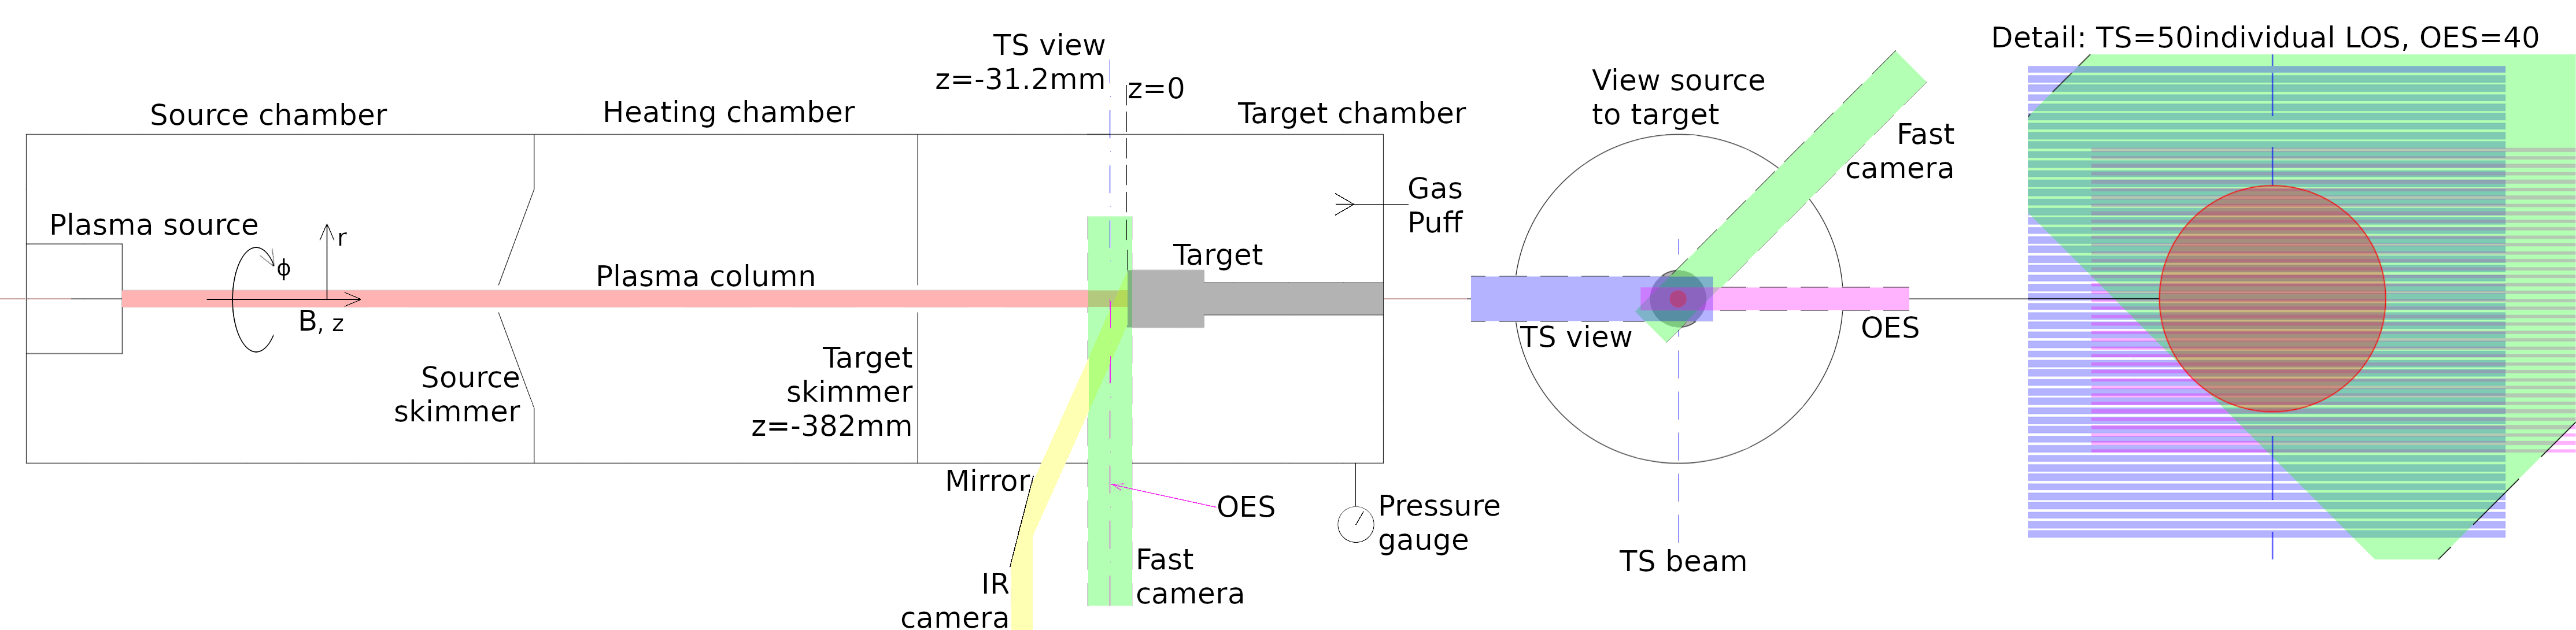
\includegraphics[width=\linewidth,trim={30 0 0 0},clip]{Chapters/chapter3/figs/layout_5.png}
	\caption{Schematic of Magnum-PSI linear plasma machine. $z=0$ corresponds to the surface of the target, Thomson scattering and Optical emission spectroscopy are located at $z=-31.2$mm. The TS view is composed of 50 evenly spaced LOS orthogonal to the plasma column while the OES one of 40. The fast camera has a radial view of the plasma through a lateral viewport of the vacuum vessel of diameter $\sim$75mm. The IR camera has a similar radial view that is converted to looking at the target surface by a mirror outside the target chamber. The mirror angle can be adapted to maintain the view of the target when moved in $z$.}
	\label{fig:layout}
\end{figure}


\subsection{Experimental conditions}\label{Experimental conditions}

In \autoref{tab:table1} are indicated the experimental conditions used on Magnum-PSI for this work, with the indication of the type of discharge based on the light emission as it will be defined in \autoref{Fast camera}. ID 1-4 are referred to as weak pulses: the magnetic field intensity is lower so the steady state and ELM-like pulse input energy is spread over a larger area, making it easier for the background gas to dissipated its energy, and the energy in the capacitor banks is also lower. ID 5-10 are conversely referred to as strong pulses, with stronger magnetic field and higher capacitor bank energy.



\begin{table}[!ht]
\small
\begin{tabular}{ | >{\centering}m{01em} | >{\centering}m{1.3cm}| >{\centering}m{1.3cm} | >{\centering}m{1.3cm} | >{\centering}m{2.0cm} | >{\centering}m{1.8cm} | >{\centering}m{2.4cm} | >{\centering}m{1.9cm} | } 
  \hline
  ID & capacitor voltage [V] & capacitor energy [J] & Magnetic field [T] & Target chamber $H_2$ feeding [slm] & Target chamber pump speed [\%] & Steady state neutral pressure in target chamber [Pa] & Stage (defined in \autoref{Fast camera}) \tabularnewline 
  \hline
  1 & 370 & 10.3 & 0.6 & 0 & 82 & 0.223 & 1 \tabularnewline 
  \hline
  2 & 370 & 10.3 & 0.6 & 0 & 25 & 0.385 & 1\tabularnewline
  \hline
  3 & 370 & 10.3 & 0.6 & 10 & 25 & 5.991 & 2/3\tabularnewline
  \hline
  4 & 370 & 10.3 & 0.6 & 20 & 25 & 10.956 & 3\tabularnewline
  \hline
  5 & 800 & 48.0 & 1.3 & 0 & 82 & 0.296 & 1\tabularnewline
  \hline
  6 & 800 & 48.0 & 1.3 & 0 & 25 & 0.516 & 1\tabularnewline
  \hline
  7 & 800 & 48.0 & 1.3 & 5 & 25 & 4.370 & 1/2\tabularnewline
  \hline
  8 & 800 & 48.0 & 1.3 & 10 & 25 & 8.170 & 2\tabularnewline
  \hline
  9 & 800 & 48.0 & 1.3 & 15 & 25 & 11.847 & 2\tabularnewline
  \hline
  10 & 800 & 48.0 & 1.3 & 20 & 25 & 15.040 & 2\tabularnewline
  \hline
\end{tabular}
  \caption{Table of the experimental conditions of Magnum-PSI for the experiments presented in this work. Common parameters are: source current 140A, 31.2mm target to OES/TS distance,TZM (a molybdenum alloy) target. ID 1-4 is referred to as weak pulses conditions while ID 5-10 are referred as strong pulses. The stages definition will be given in \autoref{Fast camera}.}
  \label{tab:table1}
\end{table}

\subsection{Diagnostics}\label{Diagnostics}

Here the diagnostics employed in this study will be introduced. Some can observe individual ELM-like pulses while other only a limited part of it, so a sampling strategy was adopted to reconstruct the full behaviour of the ELM-like pulse. More detail in \autoref{Sampling strategy}.

The results from the diagnostics used in the experiments are described in the following sections:
\begin{enumerate}
    \item[\ref{Role of molecular assisted reactions}] Jarell-Ash, Czerny-Turner spectrometer OES: Hydrogen atomic line emission (Balmer serie $p=4-8 \rightarrow 2$)
    \item[\ref{Fast camera}] Vision Research Phantom v12.1 CMOS camera: axial and radial view of the plasma
    \item[\ref{Thomson scattering}] Thomson scattering (TS): electron temperature and density
    \item[\ref{IR camera}] Infrared (IR) camera FLIR SC7500MB: target temperature (used with calibration from FAR-Associate Spectro Pyrometer FMPI)
    \item[\ref{Balance over the plasma column}] Power source (ADC): temporal variation of the power delivered to the plasma
\end{enumerate}

\subsubsection{Optical emission spectrometer (OES)}\label{Optical emission spectrometer}

The main component is a Jarell-Ash spectrometer connected to a fibre optic bundle with 40 individual cores that view the plasma radially with a resolution of 1.06mm, individual line of sight (LOS) width of $\sim$1mm. See the OES LOS in the target chamber in \autoref{fig:layout}, further detail from Barrois. \cite{Science2017}

Before this work was conducted the camera connected to the spectrometer was a Princeton Instruments PIXIS 2048B, with a shutter speed of the order of seconds. In order to obtain information on the behaviour during the pulse this camera was replaced in 2019 by the author and Gijs Akkermans with a Photometrics Prime95B 25mm RM16C with a minimum integration time of $20\mu s$. The camera has a CMOS sensor with rolling shutter, meaning the exposure of one row happens after the previous row is completed, forcing to accumulate data on multiple ELM-like pulses to reconstruct the full brightness profile. Details on how to sample all stages of the ELM-like pulse so that to obtain a coherent picture are shown in \autoref{Sampling strategy} while the steps from raw images to line emissivity are detailed in \ref{OES data interpretation}. The sensitivity calibration was done via a Labsphere as explained extensively by Barrois. \cite{Science2017} During the experiments was recorded hydrogen Balmer line emission $p=4-\infty \rightarrow 2$, with lines $p=4-8 \rightarrow 2$ considered having a sufficient signal to noise ration and being here used.

\subsubsection{Fast Camera}\label{Fast Camera1}
A Phantom v12.1 CMOS camera is installed such that it has a radial and axial view of the plasma coming from the source (left) and directed to the target (right). The view is through a lateral viewport of the vacuum vessel so the useful FOV is limited to a diameter of $\sim$75mm (see \autoref{fig:SS}, \ref{fig:ELM1}.) The camera records visible light and it’s not used to deliver quantitative information but it is very useful to establish the qualitative behaviour of the plasma. The frame rate used was 67kHz, enough to resolve individual ELM-like pulses ($\sim$1ms in duration, 67 frames). The information from multiple pulses was then averaged. Thanks to this diagnostic it is possible to identify distinct regimes that manifest by increasing the neutral pressure in the target chamber and therefore increasing the level of detachment.
\subsubsection{Thomson scattering (TS)}\label{Thomson scattering1}
Thomson scattering (TS) is a diagnostic that allows to measure $T_e$ and $n_e$ by firing a laser beam in the plasma and collecting the scattered light. 50 LOS are measured simultaneously in the radial direction (in the same plane as OES as shown in \autoref{fig:layout}) to reconstruct the profile of the plasma. In Magnum, TS can be used for steady state plasmas but also for time dependent measurements, albeit with reduced performance. For this campaign the system was used in time dependent mode with $50\mu s$ time resolution and integration time, with an uncertainty $<3\%$ for electron density and $<10\%$ in electron temperature for $n_e>2.8 \cdot 10^{20} \#/m^3$. The time between consecutive measurements must be equal to the laser frequency, 10Hz, thus forcing to accumulate data on multiple pulses to reconstruct the whole time evolution. \cite{VanDerMeiden2012} Details on the sampling strategy is given in \autoref{Sampling strategy}.
\subsubsection{IR camera}\label{IR camera1}
This data is collected by a FLIR SC7500MB infra red camera that aims at the surface of the target in the wavelength range $3.97-4.01 \mu m$. The camera view is directed towards the target by a mirror and enters the target chamber from a port upstream from the target as shown in \autoref{fig:layout}. The temperature calibration is performed with a dedicated FAR-Associate Spectro Pyrometer. The frame rate is about 3kHz, that corresponds to $\sim$3 frames per ELM-like pulse and integration time was set to $100 \mu s$. To increase the confidence on the measurements the records for multiple ELM-like pulses are overlapped and averaged once the target reached a thermal steady state in a similar fashion as done by Li. \cite{Li2020} The IR camera results are in the form of 2D the temperature profile on the target over time. Due to differences in the triggering system it is not possible to directly relate IR camera time with OES or TS so this results are used independently.
\subsubsection{Power supply}\label{Power supply}
The steady state power supply regulates the DC plasma source voltage such that its current is equal to the set point. In parallel is connected a capacitor bank composed of 28 individual sections consisting of an inductor (L=160$\mu$H) and a capacitor (C=150$\mu$F). The energy stored in each capacitor (shown in \autoref{tab:table1}) is given by $\frac{1}{2}CV^2$. These can be individually controlled such to charge to a set voltage and discharge at a set time. The current released by the capacitor will be additional to the steady state one. The voltage and current at the plasma source are recorded and data from multiple ELM-like pulses is overlapped to compensate for small differences in each capacitor/inductor pair in a similar fashion as done for the IR camera. The energy transferred into plasma energy was measured to be 92\% of the electrical energy dissipated at the plasma source during ELM-like pulses.\cite{Morgan2014} Some of the energy can additionally be dissipated in the volume between source and the target skimmer in the source and heating chamber. The pressure in these is maintained as low as possible via differential pumping to reduce interaction with cold gas and energy losses. Energy losses due to the interaction of the plasma with source and target skimmers are here neglected.
%The source and targte skimmers are estimated, from the steady state increase of cooling water temperature, to absorb $\sim$10\% and $<$0.2\% of the input energy respectlyvely.


The results that can be gathered by the examination of the individual diagnostic data, without further cross comparison will now be presented. The Fast camera will be used to understand the spatial behaviour of the pulse, the level of detachment and to distinguish the influence of increasing neutral pressure on the burn through of the pulse. Thomson scattering allows to measure the main plasma properties so that the plasma pressure losses can be compared with target chamber neutral pressure. The target temperature allows to determine the energy delivered to the target by the ELM-like pulse, finding it decreasing with increasing neutral pressure until full baffling is achieved.
Then the understanding will be deepened with the use of a Bayesian technique specifically developed to interpret in a self-consistent way results from different diagnostics. This allows to quantify the relevance of molecular assisted processes compared to the molecular ones.


\section{Fast camera}\label{Fast camera}
In this section the visible fast camera brightness is used to examine the spatial distribution of the emission in the target chamber and how the ELM-like progression to the target is impacted by increasing neutral pressure. This will allow to define 3 progressive stages of detachment based on the averaged spatial brightness profile.

\subsection{Steady state}\label{Steady state}


In order to characterise the state of the plasma during the ELM-like pulse from the visible fast camera brightness, the known characteristics of a steady state plasma are shown in \autoref{fig:SS}. \cite{Akkermans2020,Perillo2019}
These images are taken with a H$\alpha$ filter with plasma in similar conditions to the ones in this work (1.2T, 120A) during an experiment by Akkermans.\cite{Akkermans2020} Because of the presence of the filter the images are effected by blur.

\begin{figure}[!ht]
    \captionsetup{labelfont={color=white}}
     \centering
     \begin{subfigure}{0.35\textwidth}
         \centering
         \vspace*{-0mm}
         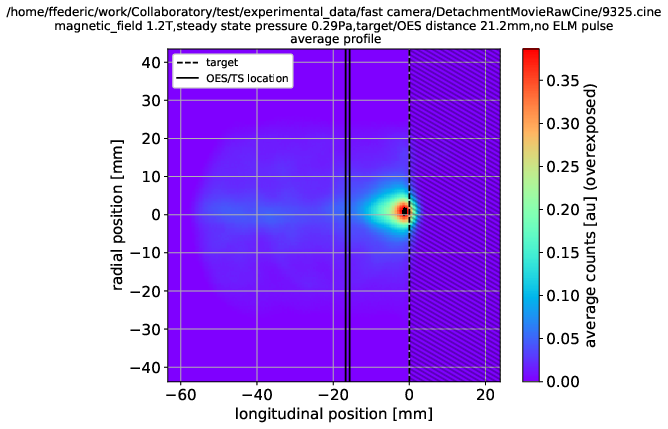
\includegraphics[width=\textwidth,trim={26 0 17 11},clip]{Chapters/chapter3/figs/fast_camera_9325.cine.png}
         \vspace*{-17mm}
         {\color{white}\caption{\phantom{weww}}\label{fig:SSa}}
     \end{subfigure}
     \hfill
     \begin{subfigure}{0.31\textwidth}
         \centering
         \vspace*{-0mm}
         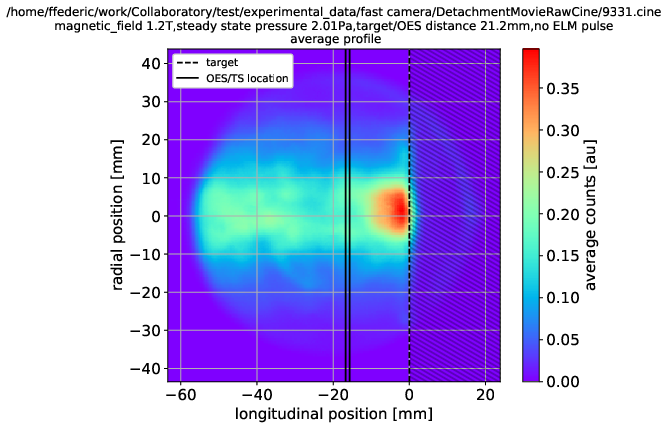
\includegraphics[width=\textwidth,trim={39 0 17 11},clip]{Chapters/chapter3/figs/fast_camera_9331.cine.png}
         \vspace*{-17mm}
         {\color{white}\caption{\phantom{wewwwww}}\label{fig:SSb}}
     \end{subfigure}
     \hfill
     \begin{subfigure}{0.31\textwidth}
         \centering
         \vspace*{-0mm}
         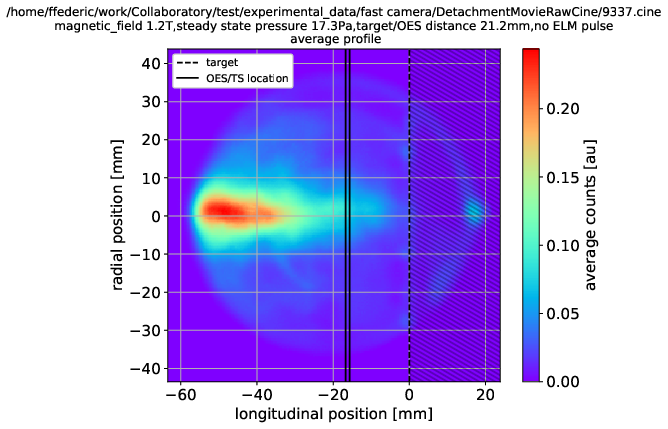
\includegraphics[width=\textwidth,trim={39 0 17 11},clip]{Chapters/chapter3/figs/fast_camera_9337.cine.png}
         \vspace*{-17mm}
         {\color{white}\caption{\phantom{wewwwww}}\label{fig:SSc}}
     \end{subfigure}
        \captionsetup{labelfont={color=black}}
        \vspace*{+6mm}
        \caption{Visible fast camera brightness corresponding to a steady state plasma in condition similar to what experimented in this work from an experiment by Akkermans\cite{Akkermans2020} (1.2T, 120A, H$\alpha$ filter present, (\subref{fig:SSa}) is effected by overexposure in the black region near the target). The target chamber neutral pressure is increased to induce detachment and corresponds to 0.29Pa (\subref{fig:SSa}), 2.01Pa (\subref{fig:SSb}) and 17.3Pa (\subref{fig:SSc}). The shaded region indicates the position of the target. The fast camera view is through a lateral viewport, giving a useful FOV of $\sim$75mm diameter.}
        \label{fig:SS}
\end{figure}

For low target chamber neutral pressure the plasma emitting region is concentrated close to the target at the centre of the plasma column. This indicates that the interactions between plasma and the background gas are weak and the plasma can flow towards the target mostly unperturbed. This is due both to the low neutral density and to the fact that the high plasma temperature typical of low target chamber neutral pressure causes further dilution. \cite{DenHarder2015} Increasing the neutral pressure the radiation in the volume increases while it decreases close to the target, indicating the volume plays an increasingly important role. By increasing the neutral pressure further the radiation becomes absent close to the target and the plasma recedes from it. The peak plasma density close to the target first increases from 1.13 to $1.98 \cdot 10^{20}\#/m^3$ from 0.29 to 2.01Pa then decreases to the point that TS measurement fails at 17.3Pa. The peak plasma temperature conversely decreases from 3.34eV to 1.53eV and becomes undetectable at 17.3Pa. That is concomitant to a monotonic loss of plasma pressure, consistent with the with the behaviour of a plasma that experience detachment caused by the increase of neutral pressure.\cite{Perillo2019} The plasma is classified as attached to the target in \autoref{fig:SSa} and \subref{fig:SSb}, while detached in \autoref{fig:SSc}.

Averaging the visible fast camera brightness over the radial direction one can obtain the profiles in \autoref{fig:SS2}, that reinforce how the main interactions of the plasma shift from close to the target to the volume of the plasma column for increasing neutral pressure. The increase in visible radiation correlates well with observations from simulations that H$\alpha$ emission is greatly increased from the detachment onset onward because of the influence of molecular reactions.\cite{Zhou2022} Established that the detachment state of the plasma can be inferred from the visible fast camera brightness we can look at the measurements during the ELM-like pulse.
\begin{figure}[!ht]
	\centering
	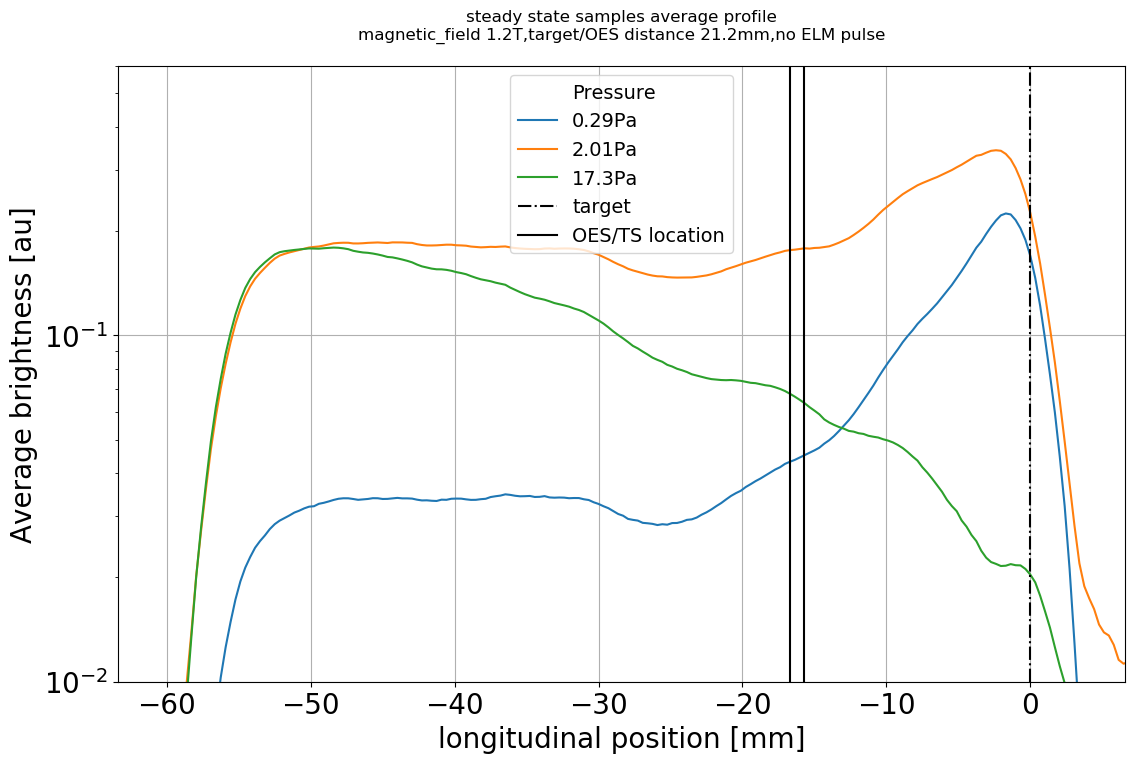
\includegraphics[width=0.7\linewidth,trim={7 0 9 45},clip]{Chapters/chapter3/figs/SS_scan4.png}
	\caption{Radial average of the visible fast camera brightness for the steady state cases in \autoref{fig:SS}. The longitudinal position axis is cut after the target. The brightness decreases towards the source as the plasma exits the field of view of the camera.}
	\label{fig:SS2}
\end{figure}


\subsection{Effect of ELM-like pulses}\label{Effect of ELM-like pulses}

The fast camera was set with a high frame rate of 67kHz and low integration time of 900ns in order to capture the bright ELM-like pulse behaviour. With this settings the brightness of the steady state is zero and only the pulse can generate counts. The ELM-like pulse lasts 0.7 to 1ms (equivalent to 67-47 frames) depending on the target chamber neutral pressure and a clear movement of a radiation front from the source to the target could not be clearly identified with this settings. In order to extract information on the behaviour across the ELM-like pulse the camera measurement is averaged in time over the time interval with non zero data. The data from a few ELM-like pulses in the same conditions is then further averaged. A sample of the results for the plasma conditions in this work are shown in figure \autoref{fig:ELM1}.

\begin{figure}[!ht]
    \captionsetup{labelfont={color=white}}
     \centering
     \begin{subfigure}{0.36\textwidth}
         \centering
         \vspace*{-0mm}
         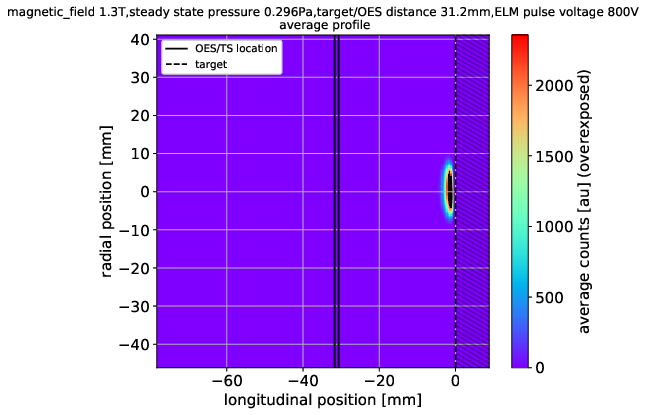
\includegraphics[width=\textwidth,trim={20 0 8 8},clip]{Chapters/chapter3/figs/fast_camera_merge_95_average3.png}
         \vspace*{-17mm}
         {\color{white}\caption{\phantom{weww}}\label{fig:ELMa}}
     \end{subfigure}
     \hfill
     \begin{subfigure}{0.31\textwidth}
         \centering
         \vspace*{-0mm}
         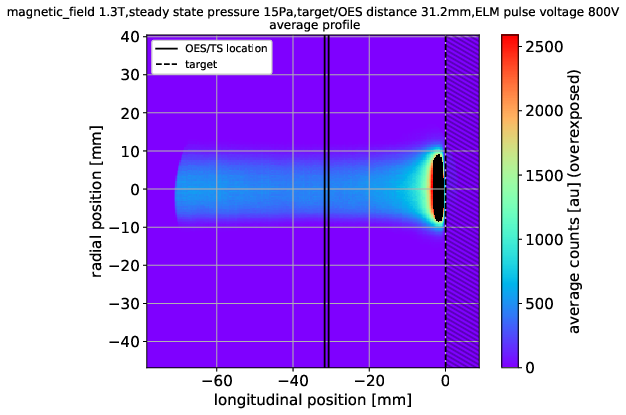
\includegraphics[width=\textwidth,trim={34 0 8 7.5},clip]{Chapters/chapter3/figs/fast_camera_merge_85_average3.png}
         \vspace*{-17mm}
         {\color{white}\caption{\phantom{wewwwww}}\label{fig:ELMb}}
     \end{subfigure}
     \hfill
     \begin{subfigure}{0.31\textwidth}
         \centering
         \vspace*{-0mm}
         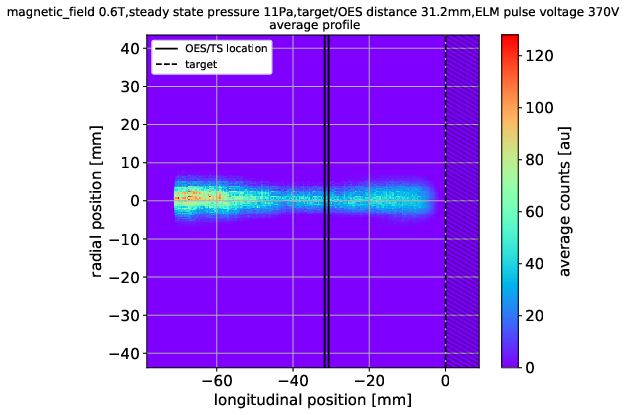
\includegraphics[width=\textwidth,trim={34 0 8 8},clip]{Chapters/chapter3/figs/fast_camera_merge_97_average3.png}
         \vspace*{-17mm}
         {\color{white}\caption{\phantom{wewwwww}}\label{fig:ELMc}}
     \end{subfigure}
        \captionsetup{labelfont={color=black}}
        \vspace*{+6mm}
        \caption{Fast visible camera images of the ELM-like obtained by averaging temporally over the pulse duration. The images show a plasma in increasingly detached and correspond to ID 5 (\subref{fig:ELMa}), 10 (\subref{fig:ELMb}), 4 (\subref{fig:ELMc}) in \autoref{tab:table1} ((\subref{fig:ELMa}) and (\subref{fig:ELMb}) are effected by overexposure in the black region near the target). The fast camera view is through a lateral viewport, giving a useful FOV of $\sim$75mm diameter.}
        \label{fig:ELM1}
\end{figure}

\autoref{fig:ELMa} corresponds to a low target chamber neutral pressure. In this conditions it is typical to register a bright emission in proximity of the target while almost nothing is visible far from it, meaning the vast majority of the interactions happens at the target while the plasma is transported, mostly undisturbed, through the bulk of the target chamber. This closely resemble what observed in \autoref{fig:SSa}, indicating that the plasma is here attached to the target. Another observation is that during the ELM-like pulse the visible fast  camera brightness close to the target increases and then decreases, while maintaining the same relative shape. This points towards the fact that the plasma is attached before, during and after the pulse. This is also confirmed by independent TS and OES measurements. From the steady state to the peak ELM-like pulse values $T_e$ rises from 5 to 9.38eV and $n_e$ from 1 to $23.7 \cdot10^{20}\#/m^3$ (see \autoref{Thomson scattering} for further details). This experimental condition is the first one encountered starting from low neutral pressure, so it is referred to a Stage 1. 

In \autoref{fig:ELMb} the neutral density is increased. The light emission in the bulk of the target chamber increases with respect to at the target and is typically quite homogeneous along the magnetic field direction. The emission closely resembles \autoref{fig:SSb}, meaning that during the ELM-like pulse the plasma is still attached to the target. This in not the case before and after, where the density is so low that TS measurements fail and no emission is visible from OES. During the ELM-Like pulse peak $T_e$ decreases to 4.61eV while $n_e$ increases to $52 \cdot 10^{20}\#/m^3$. This conditions are referred to as Stage 2.

If the neutral pressure is further increase from what causes Stage 2 to occur the baffling in the bulk of the target chamber can be so severe that the strong luminous spot close to the target might not appear. This is shown in \autoref{fig:ELMc}. In such cases the interaction of the plasma in the volume is so strong as to dissipate the ELM-like pulse almost entirely. Only luminosity in the volume is present, closely resembling \autoref{fig:SSc} that corresponds to a detached plasma, meaning the plasma is detached before, during and after the ELM-like pulse. The OES, TS, and visible fast camera brightness is measurable for a much shorter time compared to the ELM-like pulse duration ($\sim 200 \mu s$ compared to $700 \mu s$) meaning most of the ELM-like pulse energy is dissipated by the neutrals. This is further confirmed by TS as peak $T_e$ drops from 0.63 to 0.58eV and $n_e$ from 12.6 to $4.7 \cdot10^{20}\#/m^3$ increasing the neutral pressure from Stage 2 (ID 3 to 4 in \autoref{tab:table1}). This regime is referred to as Stage 3.

The information in \autoref{fig:ELM1} is summarised in \autoref{fig:ELM2} and \ref{fig:ELM3} that show the average along the radial direction of the visible fast camera brightness for varying neutral pressure for the two scans included in this work (ID 1 to 4 and 5 to 10 in \autoref{tab:table1}).

\begin{figure}[!ht]
	\centering
	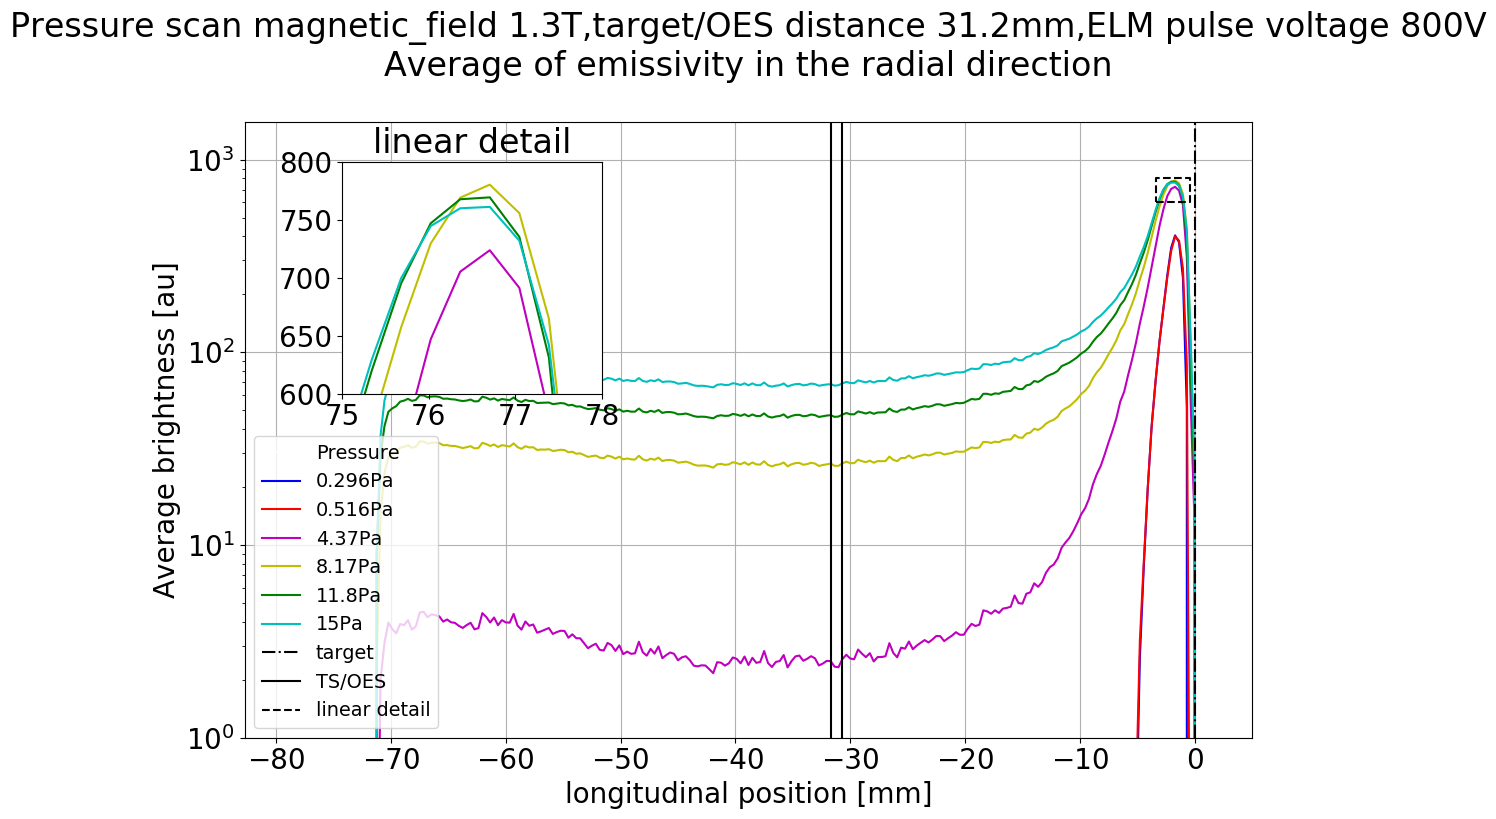
\includegraphics[width=0.7\linewidth,trim={110 0 170 85},clip]{Chapters/chapter3/figs/20.png}
	\caption{Radial and temporal average of the visible fast camera brightness for the neutral pressure scan with strong ELM-like pulses, where we observe the transition from Stage 1 to 2. (ID 5-10 in \autoref{tab:table1}).}
	\label{fig:ELM2}
\end{figure}

\begin{figure}[!ht]
	\centering
	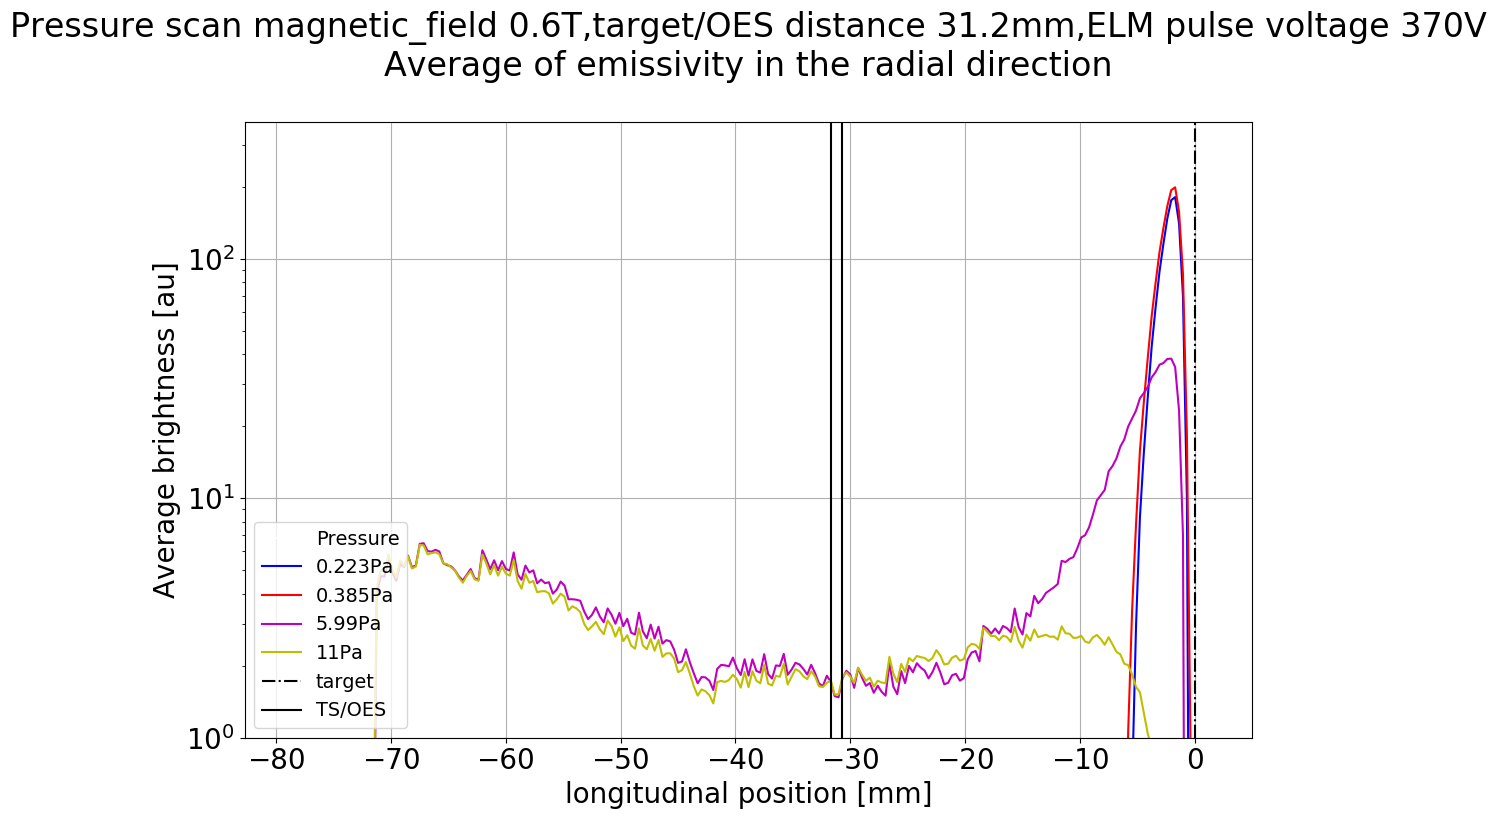
\includegraphics[width=0.7\linewidth,trim={110 0 170 85},clip]{Chapters/chapter3/figs/39.png}
	\caption{Radial and temporal average of the visible fast camera brightness for the neutral pressure scan with weak ELM-like pulses, where we observe the transition from Stage 1 to 3 (ID 1-4 in \autoref{tab:table1}).}
	\label{fig:ELM3}
\end{figure}

\autoref{fig:ELM2} corresponds to strong ELM-like pulse compared to the gas background. The emission is always peaked at the target while the emission away from it increases significantly for increasing pressure. At the two lowest neutral pressure settings the plasma is in Stage 1, it is at an intermediate state for ID7 (with a significantly lower emission in the volume then the other higher pressure cases) while it then transition to Stage 2 for ID8-10 in \autoref{tab:table1}. The brightness becomes more homogeneous along the magnetic field for increasing neutral pressure, reducing the relevance of the anisotropy. The emission at the peak initially increases with neutral pressure but, as shown in the linear detail it then start to decrease, signalling the start of the transition from Stage 2 to 3 (it must be noted, though, that the peak region is effected by saturation). It will be later shown that the peak plasma pressure does not significantly change in the transition from Stage 1 to 2, indicating that the plasma is still attached during the ELM-like pulses.
In \autoref{fig:ELM3} is shown the average of the brightness for the neutral pressure scan with weak ELM-like pulses (ID 1-4 in \autoref{tab:table1}), meaning the pulses are weak compared to the baffling of the background gas. Here we have the transition from Stage 1 (0.223 and 0.385Pa) to 2/3 (5.99Pa) and ultimately 3 (11Pa). The same trend in \autoref{fig:ELM2} continues here, with an even more uniform light emission. Note that this dataset is unaffected by saturation. The 5.99Pa case is indicated as Stage 2/3 because even if some emission comes from nearby the target, that is significantly reduced compared to the Stage 1 cases, and looking at the temporal evolution of the brightness the pulse reattaches to the target only briefly. Later analysis will show that with neutral pressure 5.99Pa no heating is delivered to the target, typical of Stage 3 rather than 2, and the plasma pressure loss is significant, indicating increasing levels of detachment.

The distinction in stages helps to discriminate between types of behaviour of the plasma and its influence on other diagnostics and the power balance. Plasmas in Stage 1 are typically correlated to low volumetric losses, high steady state target temperature and measurable steady state plasma conditions, as it will be clear from analysis of the IR camera and TS data. In Stage 2 the target is cold in between pulses but a significant heating can be provided transiently and volumetric losses dominate as power loss mechanism. In Stage 3 the lack of emission near the target coincides with negligible target heating, significant plasma losses before reaching the OES/TS location and an increased anisotropy in the plasma column.
As previously mentioned the emission is not homogeneous in the whole target chamber. Strong emission is located close to the target and even in the bulk there is a slight increase in emission moving away from the target. The anisotropy in the bulk of the target chamber, though, is weak and decreasing for increasing neutral pressure. \emph{This observation will be used in \autoref{Balance over the plasma column} to support the approximation that volumetric power losses can be considered constant from skimmer to target.}



\section{Thomson scattering}\label{Thomson scattering}


Thomson scattering measures the main plasma properties ($T_e$, $n_e$) and allows to determine the temporal evolution of the ELM-like pulse and the transfer of plasma energy from high temperature to high density for increasing neutral pressure. The data collected corresponds to plasma volumes along the path of the laser beam. The lines of sight of the light collection system are centred on the plasma column so data is collected on the plasma above and below the plasma column centre. These are averaged to return the radial profiles. A small time difference between OES and TS is also present so the raw $T_e$ and $n_e$ are resampled to match OES and smoothed to obtain the temporal and radial profiles.

\begin{figure}[!ht]
    \captionsetup{labelfont={color=white}}
     \centering
     \begin{subfigure}{0.34\textwidth}
         \centering
         \vspace*{-0mm}
         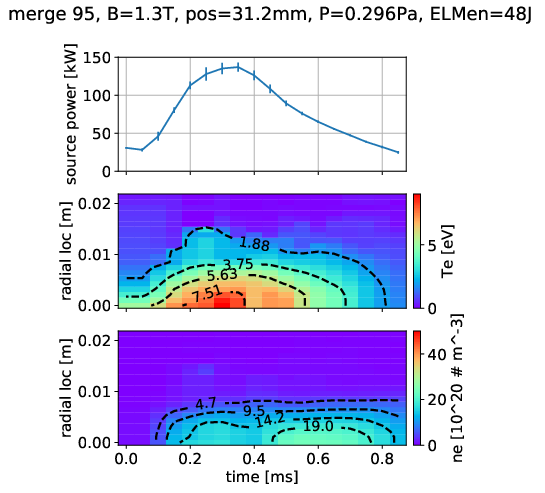
\includegraphics[width=\textwidth,trim={60 0 134 25},clip]{Chapters/chapter3/figs/pass_1_merge95_global_fit37.png}
         \vspace*{-55mm}
         {\color{white}\caption{\phantom{ }}\label{fig:TSb}}
     \end{subfigure}
     \hfill
     \begin{subfigure}{0.285\textwidth}
         \centering
         \vspace*{-0mm}
         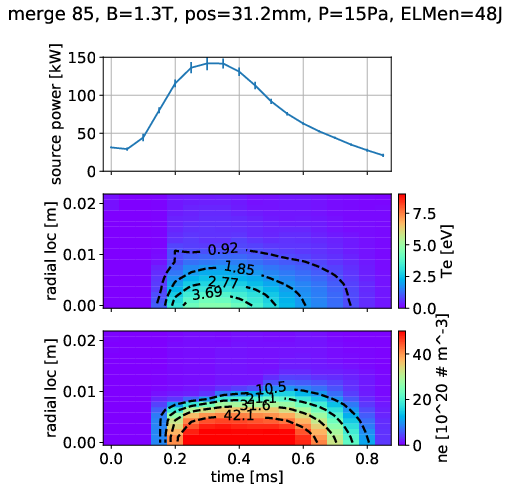
\includegraphics[width=\textwidth,trim={100 0 120 25},clip]{Chapters/chapter3/figs/pass_1_merge85_global_fit45.png}
         \vspace*{-55mm}
         {\color{white}\caption{\phantom{ }}\label{fig:TSa}}
     \end{subfigure}
     \hfill
     \begin{subfigure}{0.341\textwidth}
         \centering
         \vspace*{-0mm}
         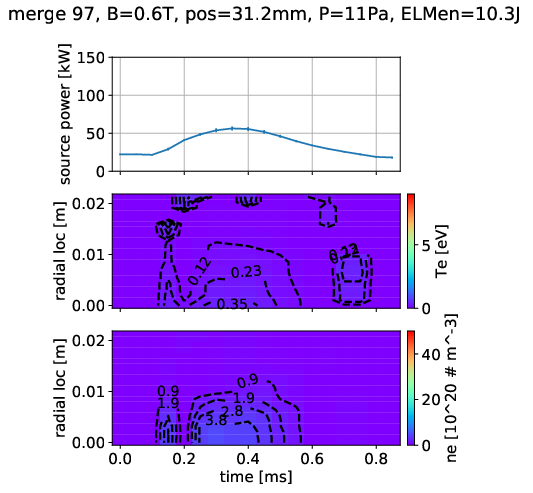
\includegraphics[width=\textwidth,trim={110 0 70 25},clip]{Chapters/chapter3/figs/pass_1_merge97_global_fit41.png}
         \vspace*{-55mm}
         {\color{white}\caption{\phantom{ }}\label{fig:TSc}}
     \end{subfigure}
        \captionsetup{labelfont={color=black}}
        \vspace*{+45mm}
        \caption{Typical source power (top), Thomson scattering $T_e$ (mid) and $n_e$ (bottom) measurement for strong pulses in Stage 1 (\subref{fig:TSb}), Stage 2 (\subref{fig:TSa}) and weak pulses in Stage 3 (\subref{fig:TSc}) (ID 5, 10, 4 in \autoref{tab:table1} respectively). TS data is smoothed over time and radius in order to match the same steps of OES.
        }
        \label{fig:TS1}
\end{figure}

In \autoref{fig:TS1} are shown typical $T_e$ and $n_e$ from TS for experimental conditions in Stage 1, 2 and 3. On top is also shown the power dissipated by the plasma source averaged over multiple ELM-like pulses and aligned with TS. As aforementioned weak pulses are obtained via a lower magnetic field and a lower energy of the pulse itself. The lower magnetic field causes the energy of the pulse to distribute over a larger area and increase the surface of contact between plasma and cold gas. The lower temperature and density also causes the neutral mean free path to increase, allowing them to penetrate deeper inside the plasma column. For strong pulses $T_e$ decreases while $n_e$ increases as the neutral pressure and the amount of gas available to be ionised increases. The steady state properties become undetectable while the time corresponding to peak density shifts earlier in time. For weak pulses and high neutral pressure peak density is at even earlier times with a very low plasma temperature.

\begin{figure}[!ht]
	\centering
	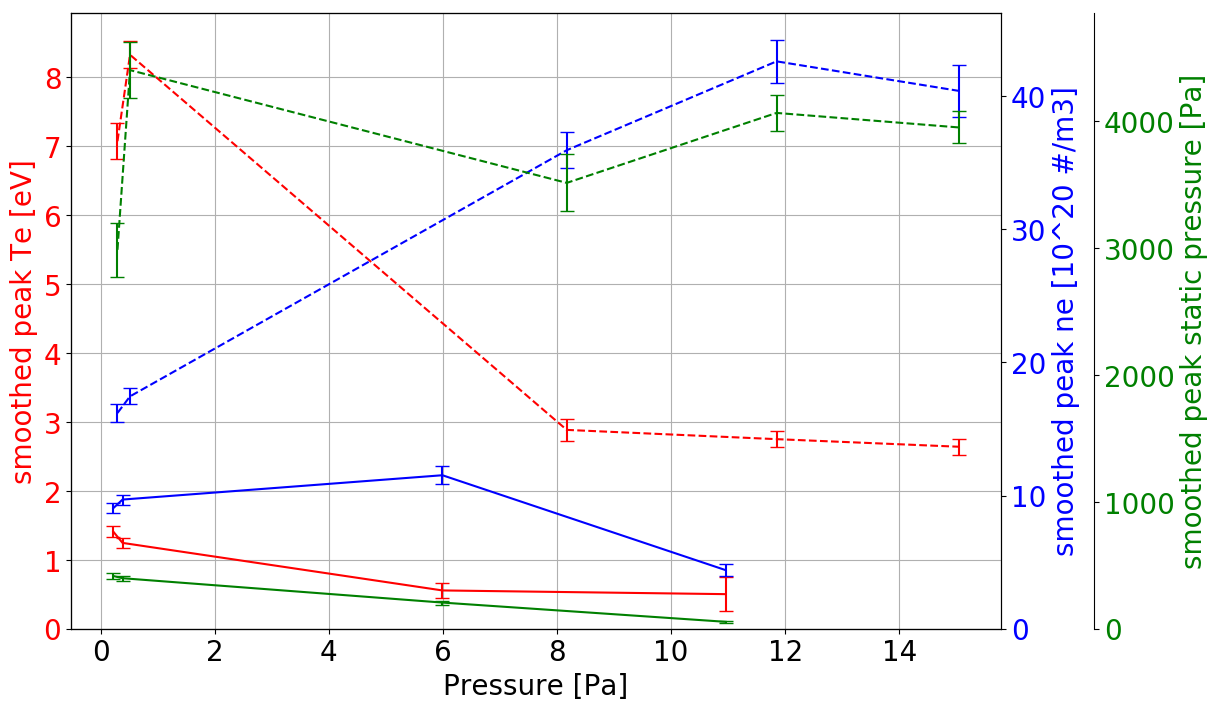
\includegraphics[width=0.7\linewidth,trim={0 0 0 0},clip]{Chapters/chapter3/figs/pure_TS_compare2.png}
	\caption{Comparison of plasma peak $T_e$, $n_e$ and $p_e$ smoothed over $700 \mu s$ for a neutral pressure scan with strong pulses (dashed lines, B=1.3T, pulse energy=48J), corresponding to \autoref{fig:ELM2} and weak (solid lines, B=0.6T, pulse energy=10.3J), corresponding to \autoref{fig:ELM3} (ID 5-10 and 1-4 respectively in \autoref{tab:table1})}
	\label{fig:TS2}
\end{figure}

A comparison of the peak $T_e$, $n_e$ and $p_e$ ($=n_e2T_e/k_B$) smoothed over $700 \mu s$ is shown in \autoref{fig:TS2}. For strong pulses $T_e$ decreases while $n_e$ increases as the neutral pressure and the amount of gas available to be ionised increases. Only the maximum neutral pressure achievable is high enough to cause a decrease of $n_e$, indicating that the plasma is starting to transition to a detached state also during the ELM-like pulse. This trend can be seen also in the static plasma pressure, that remains at similar levels as the neutral pressure increases. If it could have been further increased the plasma pressure would have likely kept decreasing as both $n_e$ and $T_e$ would. Similar trends can be seen for weak pulses too, but $n_e$ starts decreasing at much lower neutral pressure, indicating that it is easier for the gas to dissipate the plasma energy. In the highest pressure case the plasma is significantly depleted in the volume before reaching the TS location, causing the TS measurement itself to fail except at the very peak of the ELM-like pulse, and not be representative of the whole plasma column. This situation corresponds to an ELM-like pulse in Stage 3 as defined before.

In summary increasing the neutral pressure (ID 5-10 in \autoref{tab:table1}) the plasma transitions from Stage 1 to Stage 2: the energy losses before reaching the TS measuring location increase but the ELM-like pulse energy is still enough to maintain the plasma pressure constant. Further increasing the neutral pressure (ID 1-4 in \autoref{tab:table1}) the energy losses keep increasing and $n_e$ as well as $p_e$ decrease transitioning to a detached plasma in Stage 3.

% \begin{figure}[!ht]
% 	\centering
% 	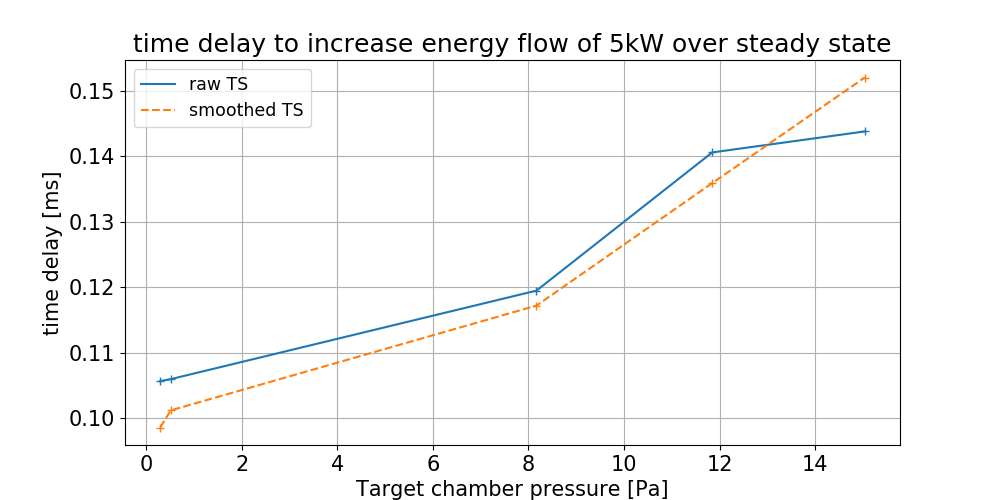
\includegraphics[width=\linewidth,trim={30 0 30 41},clip]{Chapters/chapter3/figs/image512.png}
% 	\caption{Time delay of a small variation (5KW) of the energy flow reaching the measurement location above steady state caused by the increase in neutral pressure for strong pulses (ID 5 to 10 in \autoref{tab:table1})}
% 	\label{fig:TS3}
% \end{figure}

% From TS it is also possible to show the presence of detachment and a gas buffer from its effect on the ELM-like pulse burn through, slowing it down. Assuming the plasma flows at sound speed the energy flow rate can be calculated (see \autoref{eq:plasma_column9}) and the time at which a it surpasses a threshold corresponding to a small variation over the steady state level found. This is shown in \autoref{fig:TS3}: the time gradually increases from low to high neutral pressure. Considering there is no significant effect of the neutral pressure on the power input profile, this indicates that the high temperature plasma from the source takes longer to reach the target the more background gas has to be ionised.

\section{IR camera}\label{IR camera}
The IR camera returns 2D temperature profiles of the target temperature over time. Only 3 frames correspond to a single ELM-like pulse so multiple pulses are overlapped and averaged to increase the resolution aligning all pulses peak as done by Li.\cite{Li2020} To avoid being affected by thermal transients only the last 150 of the 300 pulses within every scan is considered (see \autoref{Target temperature profile interpretation} for details). From this data the time dependent peak temperature and the shape of the effected region are extracted. These are used to show that the ELM-like pulse energy delivered to the target decreases with increasing neutral pressure to the point of being negligible therefore achieving the baffling of the ELM-like pulse.


\begin{figure}[!ht]
     \centering
     % \hspace{+11mm}
     \begin{subfigure}{0.45\linewidth}
         \centering
         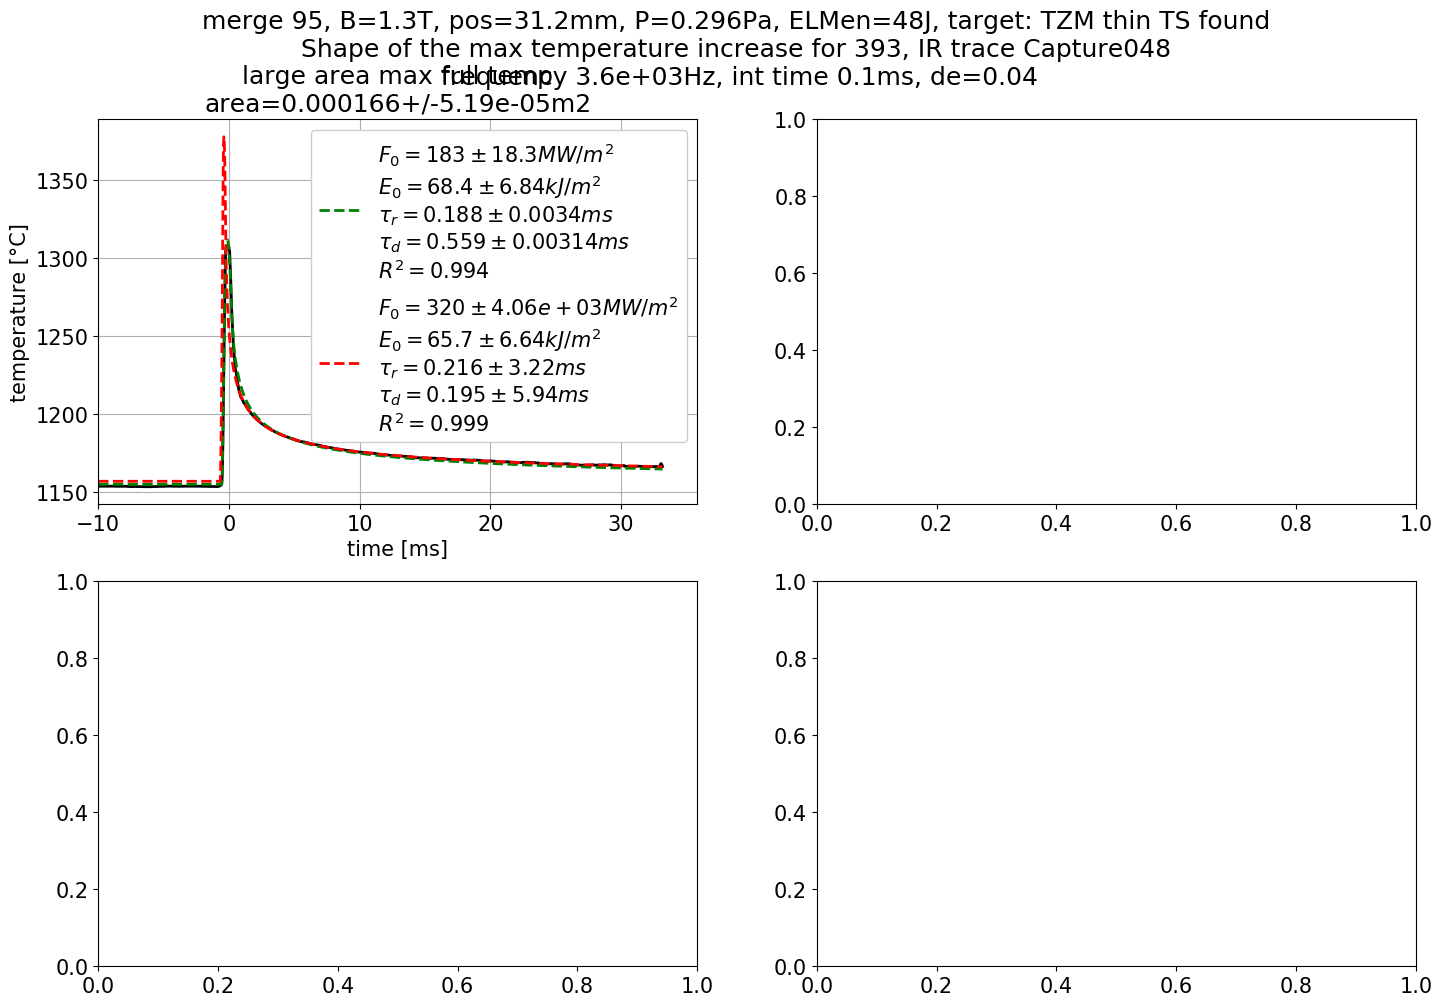
\includegraphics[width=\textwidth,trim={6 322 535 65.5},clip]{Chapters/chapter3/figs/file_index_393_IR_trace_Capture048_44.png}
         \vspace{-20mm}
         \caption{\phantom{wewwwwwwwwwww}}
         \label{fig:IR1a}
         %{\color{white}\caption{\phantom{wew}}\label{fig:TSa}}
     \end{subfigure}
     \hfill
     \vspace*{+12mm}
     \hfill
     \centering
     \begin{subfigure}{0.45\linewidth}
         \centering
         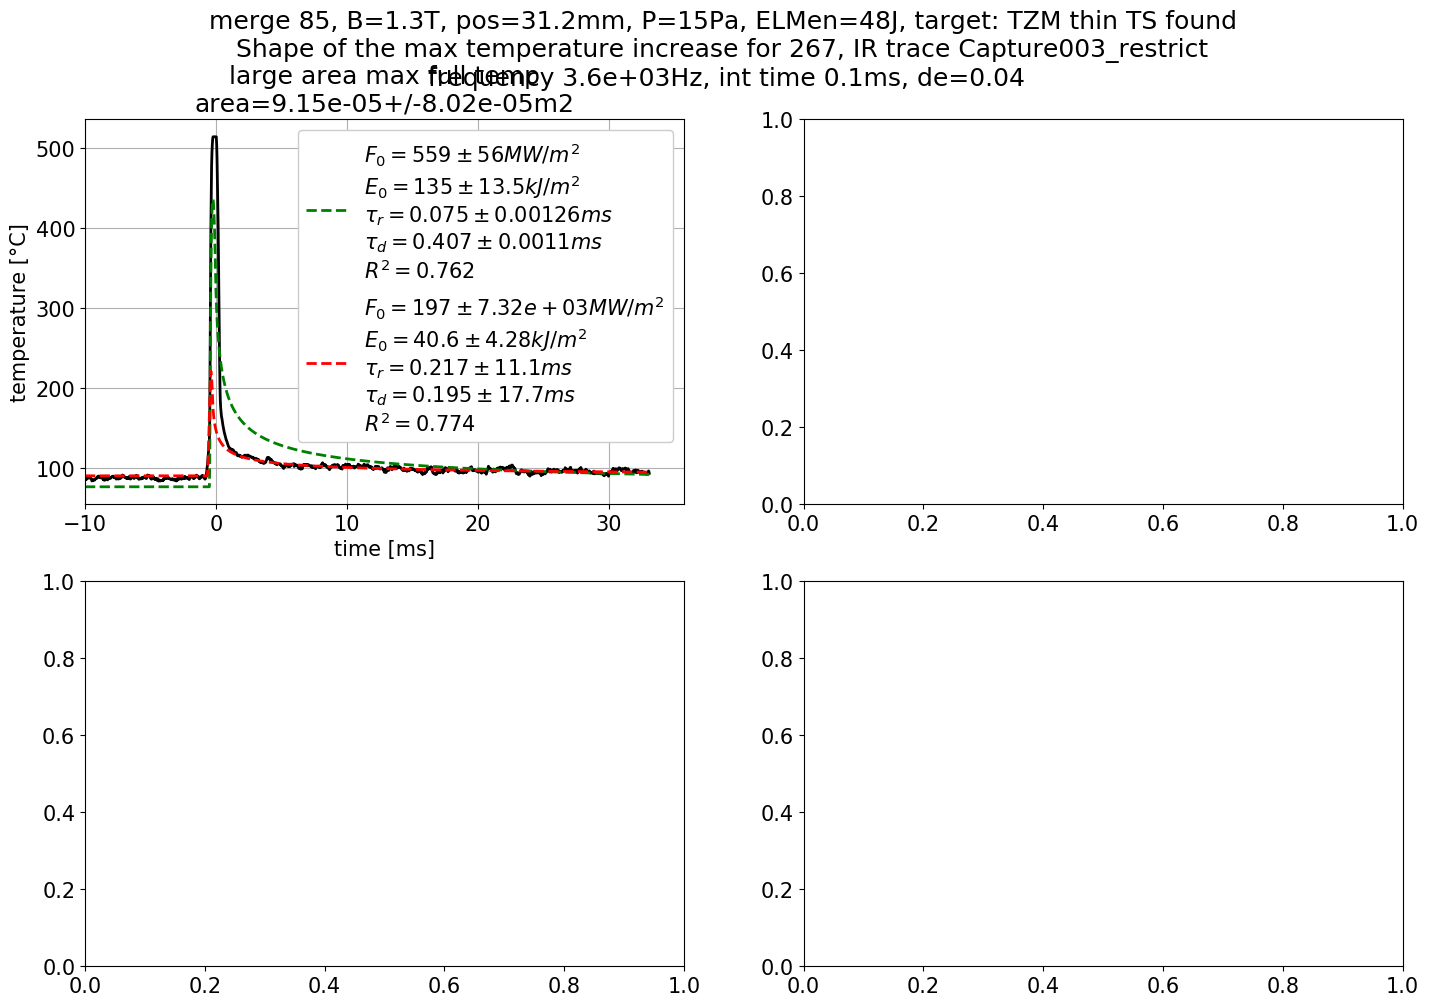
\includegraphics[width=\textwidth,trim={6 322 535 65.5},clip]{Chapters/chapter3/figs/file_index_267_IR_trace_Capture003_restrict_44.png}
         \vspace{-20mm}
         \caption{\phantom{wewwwwwwwwwww}}
         \label{fig:IR1b}
         %{\color{white}\caption{\phantom{wew}}\label{fig:TSb}}
     \end{subfigure}
        % \vspace{+10mm}
        \caption{Comparison of the measured and fitted time dependence of the peak target temperature: (\subref{fig:IR1a}) Stage 1 case, (\subref{fig:IR1b}) Stage 2 case (ID 5 and 10 in \autoref{tab:table1} respectively). The black curve is the target peak temperature The green dashed line (color online only) is the temperature fit using the entire temperature curve. The red dashed line corresponds to fitting the temperature only for the time after 1.5ms after the temperature peak. The curve is then plotted over the entire time domain using the fit parameters. In both cases the analytical model used is Model3 (\autoref{eq:triang} in \autoref{Target temperature profile interpretation}). The fit parameters are shown in the figure legend.}
        \label{fig:IR1}
\end{figure}

To estimate the energy delivered to the target the cooling curve is fitted with an analytical solution of the heat transfer equation. Various analytic solutions are available with different degrees of sophistication of the heat source time and spatial profile. It’s important to keep in mind that the quantity of interest is an estimation of the total energy density [$J/m^2$] of the heat absorbed by the target from the ELM-like pulse. The analytical solutions considered have the following power density profiles in time and space:

\begin{itemize}
    \item[Model1] a temporally square wave delivered uniformly on a semi infinite plane as described by Behrisch \cite{Behrisch1980}, commonly used in tokamaks to asses the impact of ELMs because of the large extension of the wetted area.
    \item[Model2] a temporally square wave delivered by a spatially Gaussian beam using a solution from Bäuerle \cite{Bauerle2011,Yu2016} and
    \item[Model3] a temporally triangular wave delivered by a spatially Gaussian beam using methods from Bäuerle that better reproduce the Magnum-PSI conditions.
\end{itemize}
All the above analysis methods return similar values for the total energy density delivered to the target by each ELM pulse (details of the the comparison of the various techniques are given in \autoref{Target temperature profile interpretation}). The total energy delivered to the target by the ELM-like pulse is then obtained by multiplying the peak energy density ($E_0$) by the affected area found by fitting the temperature profile after the pulse with a Gaussian profile. In \autoref{Target temperature profile interpretation} the MSC.Marc/Mentat® non linear FEM suite was used to reproduce a heat pulse as close as possible to the typical experimental conditions in terms of temporal and spatial variation and temperature dependent material properties. It was found that fitting the temperature after 1.5ms from the peak temperature returns a value of energy delivered within $\pm10\%$ of the real one. It was also found that an uncertainty of $\mp1.5ms$ in the time corresponding to the temperature peak translates to a $\pm10\%$ variation of the energy detected. This translates to a total uncertainty from the method of about $\pm20\%$, good enough for our purposes.

Typical time dependent peak temperatures are shown in \autoref{fig:IR1}. The traces presents a sharp peak followed by a slow cooling period. This fast peak can be caused by emission from the plasma (prompt emission) or an actual temperature increase of the target. For low target chamber neutral pressure the peak temperature matches well with the analytical model: sudden heating of a very thin layer of the surface of the target then the heat quickly redistributes over a larger thickness and radius, being then more slowly dissipated to the actively cooled back plate.\cite{Li2020,Morgan2020} In high neutral pressure conditions the peak is still present but it is inconsistent with the following slower cooling. The profiles are fit with Model3, fitting for all times or only the time 1.5ms after the peak. For the Stage 1 case both fits return similar energy values and, most importantly, both fit well the curve for t$>$1.5ms. This is not the case in Stage 2, where the fit for all time fails appreciably. This demonstrate the inconsistency between the temperature peak and the slowly decreasing curve in high neutral pressure conditions. We attribute the enhanced peak to prompt IR line or continuum emission from the plasma (some hydrogen molecular lines lie inside the band allowed by the IR camera filter\cite{Sternberg1989}). This is further reinforced by examining the spatial temperature distribution at the peak compared to afterwards. Further details on this and other aspects of the estimation of the energy delivered to the target are given in \autoref{Target temperature profile interpretation}. The OES could be used to differentiate between emission from the plasma column and then reflected by the target or emission from its immediate vicinity but because of the different wavelength ($3.97-4.01\mu m$ vs $0.32-0.52\mu m$) a direct comparison is not possible. In order to avoid possible misinterpretations only the temperature after 1.5ms from the peak is used rather than the peak itself. 

\begin{figure}[!ht]
	\centering
	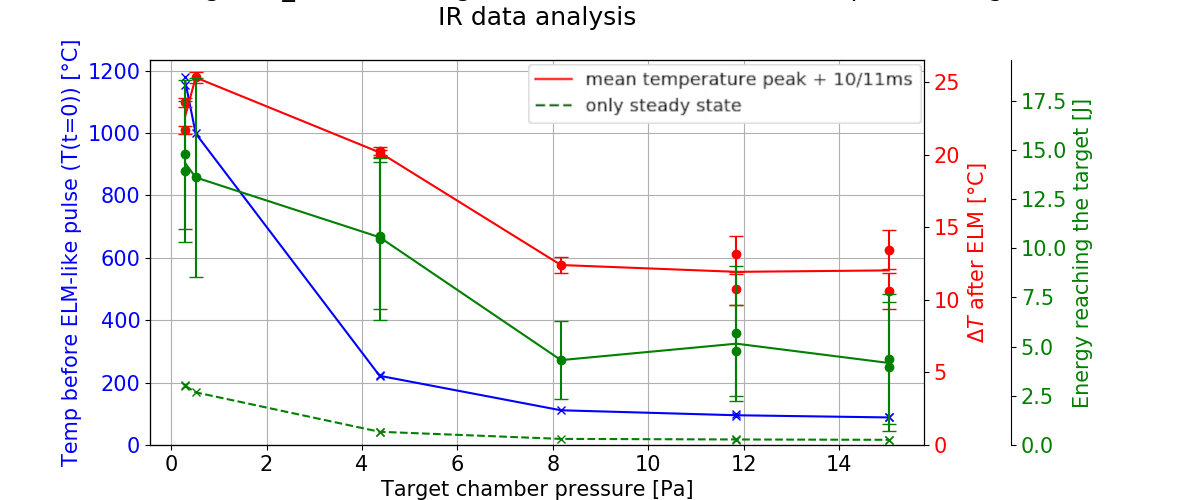
\includegraphics[width=0.9\linewidth,trim={35 0 75 22},clip]{Chapters/chapter3/figs/image515_2.png}
	\caption{Results of analysis of the IR data for the variations in target chamber neutral pressure. In this figure we focus on the case of strong pulses (48J at the source) and higher magnetic field that yields higher plasma pressure background plasma (ID 5 to 10 in \autoref{tab:table1}). Analyzed data displayed are: target temperature before the ELM (blue), temperature increase during the ELM (red), ELM energy reaching the target (solid green) estimated with Model3 fitted after 1.5ms of the temperature peak and the steady state heat flux (dashed green).}
	\label{fig:IR2}
\end{figure}
\begin{figure}[!ht]
	\centering
	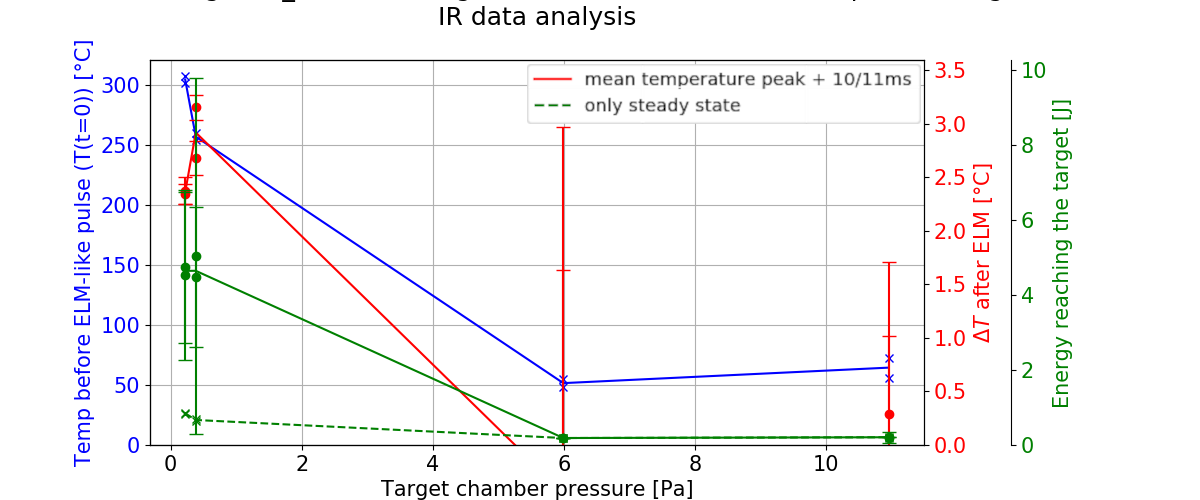
\includegraphics[width=0.9\linewidth,trim={35 0 80 30},clip]{Chapters/chapter3/figs/image516_2.png}
	\caption{Results of analysis of the IR data for the variations in target chamber neutral pressure. In this figure we focus on the case of weak pulses (10.3J at the source) and lower magnetic field that yields lower plasma pressure background plasma (ID 1 to 4 in \autoref{tab:table1}). Analyzed data displayed are same as \autoref{fig:IR2}.}
	\label{fig:IR3}
\end{figure}

In \autoref{fig:IR2}, for strong pulses, and \autoref{fig:IR3}, for weak ones, are shown the results from the analysis of the target temperature. In blue is indicated the temperature prior the ELM-like pulse, that decreases for increasing target chamber neutral pressure as it would be expected for increasing volumetric losses in the target chamber and increasing level of detachment in steady state. In red is indicated the average temperature increase 10 to 11ms after the peak. This is done to mitigate the uncertainty in the time of the real temperature peak, hidden by the prompt emission for high neutral pressure cases. This indicates that at low neutral pressure a large portion of the energy of the ELM-like is absorbed by the target, while it is more and more dissipated in the volume for increasing target chamber neutral pressure. In green are indicated the results from the analytical model. In solid green is indicated the energy absorbed by the target calculated as mentioned above. In the extreme case of high target chamber neutral pressure and weak ELM-like pulse shown in \autoref{fig:IR3} the energy delivered to the target is negligible, indicating that the pulse energy was mostly dissipated by the gas in the target chamber. In dashed green is indicated the steady state component, always relatively small. The energy delivered decreases with fueling in a similar fashion as the temperature increase after the pulse. Most notably the energy delivered is negligible for the case with strongest baffling.

The thermal analysis allows to compare the heat fluxes due to an ELM-like pulse in Magnum with Tokamaks. A metric often used in Tokamaks to estimate effect of ELMs is the heat flux factor, defined as the energy of the ELM divided by the area in which it is delivered divided by the square root of its duration. This metric is derived by the same analytic solution for the temperature increase in Model1 and is proportional to the maximum temperature increase. The maximum heat flux factor to prevent tungsten melting is $\sim$50MJ$m^{-2} s^{-0.5}$ while $\sim$40MJ$m^{-2} s^{-0.5}$ for the molybdenum target used here. The limit to prevent cracking is about half of the melting one\cite{Pintsuk2007} with some studies indicating it as low as 6MJ$m^{-2} s^{-0.5}$ for tungsten.\cite{Linke2019}

The heat flux factor obtained in these experiments was estimated using as pulse duration the integral of the power flow from TS (assuming sonic flow and using the equation for the convected power in \autoref{Balance over the plasma column}) divided by its peak. In the strong pulses case the heat flux factor is decreased from 3.5 for p$<$6Pa to 2MJ$m^{-2} s^{-0.5}$ for p$>$6Pa, while for weak pulses from 0.4MJ$m^{-2} s^{-0.5}$ for P$<$3Pa to effectively zero for P$>$3Pa. These heat flux factors are higher than what measured in current tokamaks ($<$1.3 for JET) but much lower than what could be achieved in ITER ($\sim$600MJ$m^{-2} s^{-0.5}$ for unmitigated ELMs).\cite{Jachmich2011}

In a tokamak the connection length is of the order of tens of meters on the outer target and divertor neutral pressure can reach the Pascal range\cite{Kallenbach2018}. If the divertor is separated from the main chamber by a baffle, meaning there is a physical barrier between the divertor and the main chamber, the plasma can plug the divertor entrance and the neutrals cannot freely move between the two. The neutrals have to interact with the plasma in the SOL and (in deep detachment) the ionisation front, and the neutral pressure behind the ionisation front can be increased by more than one order of magnitude compared to that in the main chamber.\cite{Galassi2020,Pitcher2000,Niemczewski1997} In these experiments the connection length in the target chamber is 0.38m and the neutral pressure up to 15Pa. Given the the energy delivered to the target by the ELM-like pulse is reduced with neutral pressure and that tokamaks are characterised by potentially longer connection lengths and similar or higher neutral pressures behind the ionisation front, this result implies that a significant reduction of the heat flux factor in tokamaks should be possible thanks to the cold regions forming close to the target when strongly detached too. The reduction of heat flux factor and heat flux to the target with pressure and connection length could be non linear (see the higher pressure cases in \autoref{fig:IR2}) but \autoref{fig:IR3} shows that transitioning from stage 2 to 3 via volumetric losses should ultimately be possible. The viability of this method to buffer ELMs will ultimately depend on the neutral pressure required to achieve the needed buffering and its effect on the inter-ELM plasma. Configurations like the super-x divertor could be the most suitable for this approach, as the ionisation front could be maintained relatively close to the x-point while a large volume with high neutral pressure can be maintained in the super-x divertor chamber. Reducing the ELM heat flux factor would improve the safety for long term operations in a tokamak, further showing the benefit of baffling and increasing the neutral chamber pressure in detached scenarios.

In summary by increasing the target chamber neutral pressure is possible to cause detachment of the steady state plasma from the target surface. From the visible fast camera brightness it is possible to identify 3 stages for the interaction between the ELM-like pulse and the background gas in the target chamber. By increasing the neutral pressure more interactions happen in the volume rather than in contact with the target, and become more homogeneous. This is true up to Stage 3, where the loss of plasma in the volume becomes dominant. A regime was found for which the gas in the target chamber can effectively prevent the ELM-like pulse to influence the target.
These results are obtained using one diagnostic at the time. To gain more insight the OES data will be combined with TS and the input power source measurement within a Bayesian framework. The purpose is to identify which processes are more relevant in the increase of removed energy in the volume for increasing level of steady state detachment, driven by target chamber neutral pressure, and possibly their evolution in time.

\section{Role of molecular assisted reactions}\label{Role of molecular assisted reactions}
In this section we describe an analysis technique that merges information from different diagnostics on Magnum-PSI data to gain more insight on the dominant atomic and molecular processes during an ELM-like pulse. A significant aspect of this analysis is the inclusion of the molecular species $H_2$, ${H_2}^+$ or $H^-$. These species interact with the plasma leading to the formation of excited hydrogen atoms, power and particle sources/sink which have a significant influence on the behaviour of deeply detached plasmas. Since the interaction of these species with the plasma causes hydrogen atomic line emission they will be referred to as molecular precursors.

The ordinary method to infer the plasma properties from Balmer emission lines is to consider that the emission from higher-p H excited states is mainly generated via electron-ion recombination (EIR), while the emission from lower excited states is generated via electron impact excitation (EIE), and molecular contributions are generally neglected for simplicity. This normally allows to determine if the plasma is ionising, recombining or in between.\cite{Potzel2012,Verhaegh2019}. Under conditions like those in this work, on the other hand, molecular contributions can be significant.\cite{Akkermans2020} Plasma molecular interactions lead to excited hydrogen atoms generally excited to low $p$ levels, and their distribution across p is similar to the one of EIE (see \autoref{Limitations due to the measured lines}). 

In order to find the set of plasma/molecule/atom characteristics ($T_e$, $n_e$, $n_{H}/n_e$, $n_{H_2}/n_e$, $n_{{H_2}_+}/n_{H_2}$, $n_{{H}^-}/n_{H_2}$, one of these quantities is referred to as $\Theta_i$ while a set of 6 as $\Theta$) that best match both the line emission (from OES) and the electron temperature and density (from TS), a Bayesian approach is followed. This allows the analysis method to pool together information from different diagnostics in combination with priors from simulations as well as reaction rates to find the best match to experimental data and thus derive an understanding of the dominant processes and effects on the energy and particle balance. The main advantage of this approach is that it can not only account for all uncertainties and non linear rates, but also allows calculating the probability density function (PDF) of the quantities of interest. This implies that multiple non unique solutions, if present, can be found.

Probabilistic approaches have been used before to infer the full state of the divertor plasma in tokamaks but never during the ELM burn through.\cite{Verhaegh2017,Verhaegh2020,Bowman2020} First, the parameter space of $\Theta$  is defined, forming a regular grid. The range and samples of the $\Theta_i$ parameter are defined based on Thomson scattering and other priors. Given a certain combination of parameters $\Theta$ the outputs of all the quantities of interest can then be calculated, like line emission, power and particle sinks and sources, etc. Those predicted observables can then be compared with the priors to find the probability that the calculated values match the expected ones. This comparison and the calculation of the observables depend on the specifics of the problem and the simplifications used. For the combination of parameters $\Theta$ the probability from the priors is multiplied with the probability from the comparison of the calculated and measured line emission, returning the likelihood of the particular $\Theta$. Starting with this grid one can: add individual $\Theta$ searching for the maximum of the likelihood, or refine the grid further around the best $\Theta$. A grid refinement is done here to retain a grid structure and simplify the numerical problem, done just twice to limit the computational cost and memory requirements. After the quantities of interest like, for example, terms of the power balance, can then be calculated for each $\Theta$ and their probability density function (PDF) found.

%It is very helpful to develop a certain number of parameters or ranges of parameters known as (priors). The priors are applied depending on the physics of the problem and will limit the range of a number of observables. These can then be compared to the experimental measurements to find the likelihood that a specific combination of priors was present. One can then optimize the priors to look for the combination of  with maximum likelihood, or consider a range of priors around the best ones and extract the probability density function (PDF) of any derived quantity of interest, for example, terms of the power balance.

\autoref{Balance over the plasma column} gives the full list of assumptions used to simplify the physics of the plasma of interest (from the target skimmer to the target, see \autoref{fig:layout}). In short, the plasma is considered homogeneous along its length ($z$) from the target chamber skimmer to the target within each time step, and being poloidally ($\phi$ in \autoref{fig:layout}) symmetric for a given radius ($r$). This is supported by the relatively uniform visible light emission far from the target found in Stage 1 and 2 in \autoref{Fast camera}. This means that the ELM-like pulse is not localised at a particular spatial location but happens along the whole plasma column, matching well the fast nature of the transport along field lines ($\sim$ sonic flow, $<20 \mu s$ to flow through the target chamber) compared to the changes in plasma conditions over time (changes well resolved with $50 \mu s$ time steps). The conditions at the target chamber skimmer will be considered the input to the plasma column. The conditions at the target chamber skimmer will be considered the input to the plasma column. The presence of impurities is monitored by a 6-channels Avantes AvaSpec-2048-USM2-RM survey optical emission spectrometer covering the range 299-950nm\cite{Science2017} The spectrometer's channels LOSs are in the target chamber and impurities like metals from the power source or oxygen from cooling water are only detectable in significant amounts when the plasma source fails. This shows that impurities from the source are ordinarily efficiently removed in Magnum-PSI by differential pumping. Carbon can play a significant role when graphite targets are used\cite{VanEck2013}, but this is not a concern in these experiments a TZM target was used.

The integral over the ELM-like pulse of quantities of interest, like terms of the power balance, are obtained by summing the contribution from each time step and radial location. In the following section we will explain the method used to determine the probability associated with an output at a given time and radial location.

\subsection{Analysis steps}\label{Analysis steps}

We will describe here in more detail the steps to first initialize the paramenter space based on TS and other priors (\autoref{Parameter space initialisation}). Then we will show how to compare the modelled quantities and TS with the priors to  obtain the probability of each $\Theta$ (\autoref{Prior probability distribution}). Lastly the comparison with the measured Balmer lines emission, grid refinement process and determination of the quantity of interest PDFs will be illustrated (\autoref{Bayesian analysis}). The numbering of each step corresponds with the numbers in the boxes in \autoref{fig:bayes1a}, \ref{fig:bayes1b}, \ref{fig:bayes1c}.

\subsubsection{Parameter space initialisation}\label{Parameter space initialisation}

\begin{figure}[!ht]
	\centering
	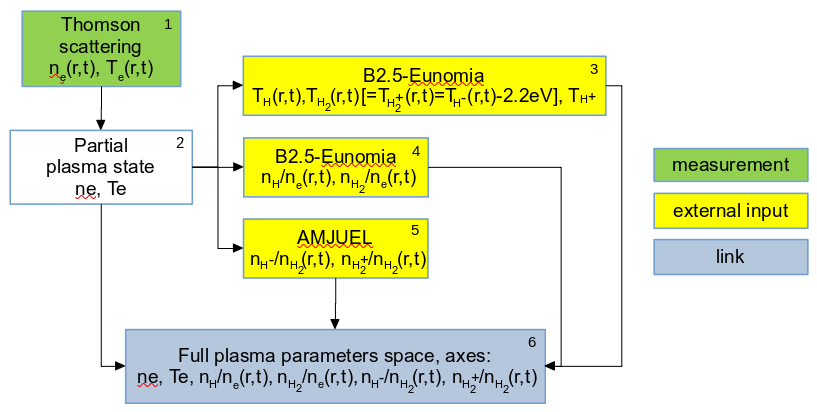
\includegraphics[scale=0.29,trim={0 0 0 0},clip]{Chapters/chapter3/figs/bayesian_steps10.png}
	\caption{Sketch illustrating how the initial guess of each parameter $\Theta_i$ is done. With \emph{link} are marked items that link different parts of the global bayesian routine together. \emph{measurement} indicate quantities measured experimentally and \emph{external input} represents inputs from simulations or reaction rates libraries.}
	\label{fig:bayes1a}
\end{figure}

% \begin{figure*}
% 	\centering
% 	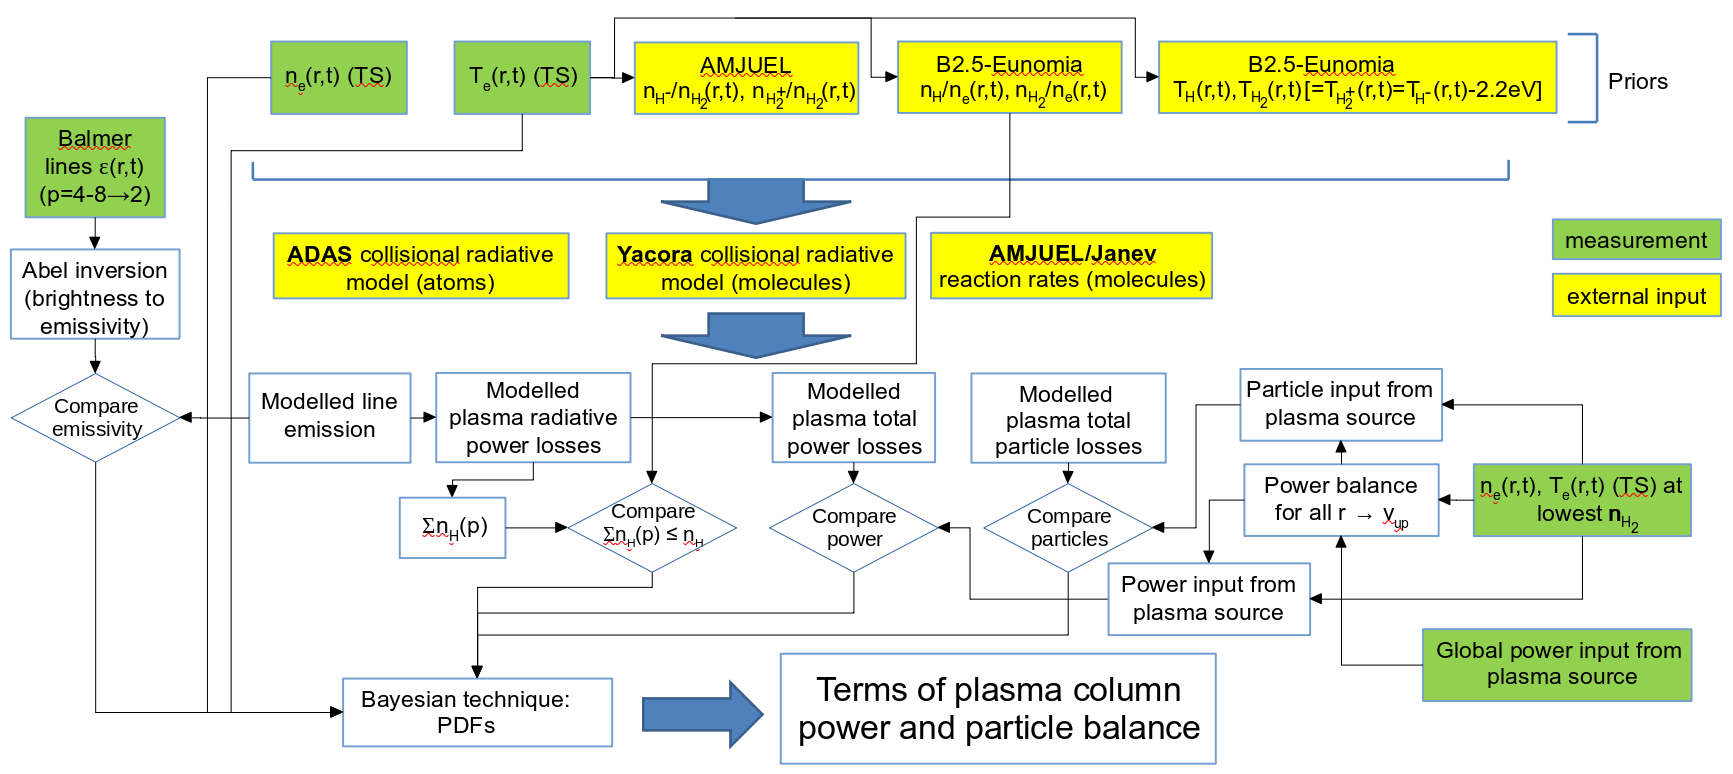
\includegraphics[width=\linewidth,trim={10 10 0 10},clip]{Chapters/chapter3/figs/bayesian_steps4.png}
% 	\caption{Sketch summarising the steps and process flow for determining the PDF of the quantities of interest for the plasma column power balance from the experimental measurement (green) and the external inputs from simulations or reaction rates libraries (yellow). \hl{from Bruce: split this plot in groups and make plots of their contents separately}}
% 	\label{fig:bayes1}
% \end{figure*}

Our Bayesian analysis first finds the range of parameters to utilize. This is shown in \autoref{fig:bayes1a}. Every point in time and radius $(t,r)$ during the ELM-like pulse is considered independently. Referring to \autoref{fig:bayes1a} the meaning of the steps are as follows:
\begin{enumerate}
    \item[1,2] \emph{Thomson scattering $n_e$(r,t), $T_e$(r,t)}: \\The measured $T_e$ and $n_e$ and their uncertainties are used to specify the range and grid elements of $T_e$ and $n_e$. From every $T_e,n_e$ combination the samples for the other $\Theta_i$ are calculated.
    \item[4] \emph{B2.5-Eunomia $n_H/n_e$(r,t), $n_{H_2}/n_e$(r,t)}: \\ We utilize B2.5-Eunomia simulations, a multi-fluid plasma code coupled with a non-linear Monte Carlo transport code for neutrals\cite{Wieggers2013,Chandra2021,Chandra2022}, to determine scalings for $n_{H_2}$ and $n_H$ with $T_e$. We utilize these scalings to obtain ranges for $n_{H_2}/n_e$ and $n_H/n_e$ (see \autoref{Priors from B2.5 Eunomia} and \ref{Priors range optimization}).
    \item[3] \emph{B2.5-Eunomia $T_H$(r,t), $T_{H_2}$(r,t)[$=T_{{H_2}^+}(r,t)=T_{H^-}(r,t)-2.2eV$], $T_{H^+}$}: \\Similarly, values of $T_H$, $T_{H_2}$ and $T_{H^+}$ are extracted from B2.5-Eunomia simulation scalings with $T_e$. Given the molecular precursor ${H_2}^+$ is predominantly generated from $H_2$ it is assumed that $T_{H_2}=T_{{H_2}^+}$. In the creation of $H^-$ from $H_2$ the ion can get some of the Frank-Condon energy of the $H_2$ bond (2.2eV per nucleon). For this reason 2.2eV are added to $T_{H_2}$ to estimate $T_{H^-}$\cite{Verhaegh2020} (see \autoref{Priors from B2.5 Eunomia}).
    \item[5] \emph{AMJUEL $n_{H^-}/n_{H_2}$(r,t), $n_{{H_2}^+}/n_{H_2}$(r,t)}: \\${H_2}^+/H_2$ and $H^-/H_2$ density ratios are calculated from the AMJUEL collection of cross sections, reaction rates and ratios \cite{Reiter2017,Reiter2005,Kotov2007} to determine the $n_{H^-}/n_{H_2}$ and $n_{{H_2}^+}/n_{H_2}$ ranges used as priors (see \autoref{Priors from AMJUEL} and \ref{Priors range optimization}).
\end{enumerate}

\subsubsection{Prior probability distribution}\label{Prior probability distribution}

\begin{figure*}
	\centering
	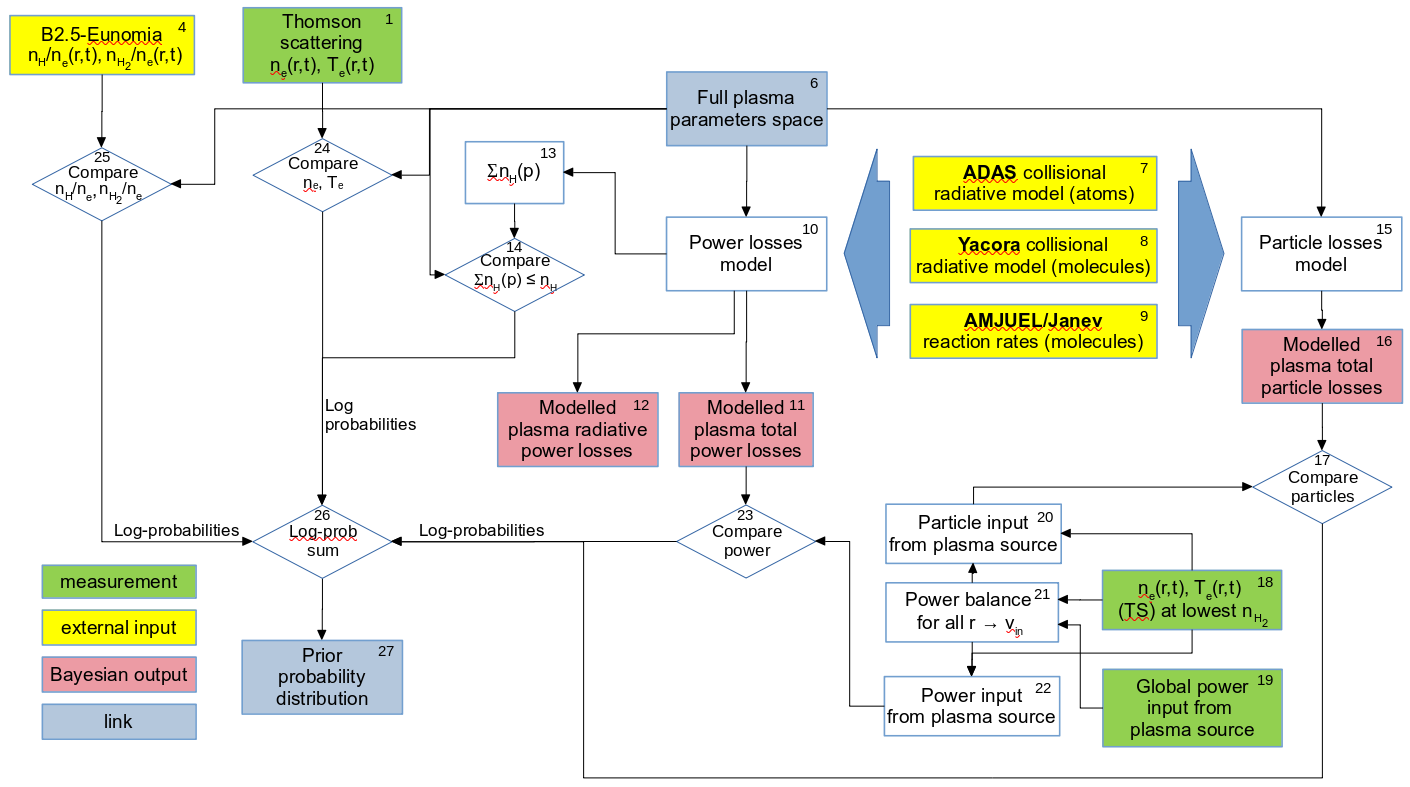
\includegraphics[scale=0.29,trim={0 0 0 0},clip]{Chapters/chapter3/figs/bayesian_steps12.png}
	\caption{Sketch illustrating how the prior probability distribution is determined given the parameter grid. \emph{Bayesian output} indicates groups of quantities that are collected for all the parameter space and with the likelihood will return their PDF.}
	\label{fig:bayes1b}
\end{figure*}

Once the initial parameter space is determined the prior probability distribution is calculated. The process for this is shown in \autoref{fig:bayes1b} and the meaning of the steps is as follows:

\begin{enumerate}
    \item[7] \emph{ADAS colisional radiative model (atoms)}: \\The ADAS collisional radiative model\cite{Summers2004,OMullane2013} is used to calculate the line emission (see \autoref{Emissivity}), the power losses (see \autoref{Power balance}) and the particle balance sources/sinks (see \autoref{Particle balance}) due to atomic processes. The reactions considered and relative coefficients are indicated in \autoref{tab:adas}. This type of analysis is fairly standardised, see for example \cite{Verhaegh2018}.
    \item[8] \emph{Yacora collisional radiative model (molecules)}: \\The Yacora collisional radiative model\cite{Wunderlich2016,Wunderlich2020} is used to calculate the line emission due to molecular precursors via the population coefficients (see \autoref{Emissivity}) and the radiative power losses (see \autoref{Power balance}). The molecular precursors that will be utilized in this analysis are $H_2$, ${H_2}^+$ and $H^-$ based on the work by Verhaegh \cite{Verhaegh2021} (see the reactions in \autoref{tab:yacora}). ${H_3}^+$ could also be considered, but its relevance is expected to be much lower than that of ${H_2}^+$ and $H^-$ so it is dropped to limit the number of variables.\cite{Verhaegh2021}.
    \item[9] \emph{AMJUEL/Janev reaction rates (molecules)}: \\The AMJUEL database and a collection of reaction rates from Janev \cite{Janev2003} is used to calculate the rate of reactions involving molecular precursors (see \autoref{tab:amjuel}, \ref{tab:janev}). The reactions rates are use then to calculate sources and sinks in the power and particle balance in the plasma column (see \autoref{Power balance}, \ref{Particle balance})
    \item[19] \emph{Global power input from plasma source}: \\The power input from the plasma source is calculated from the measurement of voltage and current on the plasma source. From a study  by Morgan\cite{Morgan2014}, 92\% of the electrical energy is transferred to the plasma during an ELM-like pulse. This value will be considered valid for each time step.
    \item[18] \emph{$n_e(r,t), T_e(r,t)$ (TS) at lowest target chamber pressure}: \\It is assumed that for the lowest pressure case the interactions between the plasma column and the background gas in the target chamber are negligible, therefore they represent the input conditions for all cases that differ only by the target chamber neutral pressure. They are referred to as $n_{e,in}, T_{e,in}$ and used to determine the input power and particle profiles (see \autoref{Balance over the plasma column}).
    \item[21] \emph{Power balance for all $r \rightarrow v_{in}$}: \\Assuming that the plasma flows from skimmer to target with the same Mach number ($M_{in}(t)$) across different radii it is possible to relate the total input power ($P_{source}(t)$) with the input conditions ($n_{e,in}(r,t), T_{e,in}(r,t)$). It is then possible to determine $M_{in}(t)$ and then $v_{in}(r,t)$. See \autoref{Balance over the plasma column} for details.
    \item[22] \emph{Power input from plasma source}: \\The maximum power input is calculated as the energy flow due to a plasma in the input conditions ($n_{e,in}(r,t), T_{e,in}(r,t)$) at flow velocity $v_{in}(r,t)$ plus the the energy associated to the depletion of the plasma at the specific neutral pressure of the experiment ($n_e(r,t), T_e(r,t)$) in one time step. See \autoref{Power balance} for details.
    \item[20] \emph{Particle input from plasma source}: \\Similarly to the previous step the maximum particle input is obtained as the input particle flow using $n_{e,in}(r,t)$ and $v_{in}(r,t)$ plus the particle flow associated with the dissipation of the plasma at the specific neutral pressure of the experiment ($n_e(r,t)$) in one time step. See \autoref{Particle balance} for details.
    \item[10] \emph{Power losses model}: \\ The power losses in the annular section of the plasma column of interest are modelled as per \autoref{Power balance}. The effect of impurities is not considered, as it is assumed that most of the impurities introduced by the plasma source anode and cathode are removed by differential pumping in the source and heating chamber.
    \item[12] \emph{Modelled plasma radiative power losses}: \\The total radiated power from the plasma column is calculated. For atomic processes ADAS coefficients are used. For molecular processes Yacora coefficients are used, summing the line emission for all possible transitions (the highest excited state considered is p=13). It is not considered the radiation caused directly by $H_2, {H_2}^+, H^-$ excited states, as it should have a negligible contribution.\cite{Groth2019}
    \item[11] \emph{Modelled plasma total power losses}: \\The total power losses are obtained by adding: total radiated power losses, net difference of potential energy from reactants to products and energy loss attributed to the heat carried away from the neutral produced by recombination. This terms and their components are part of the outputs of the Bayesian analysis.
    \item[23] \emph{Compare power}: \\The modelled net power losses are compared to the power input previously inferred. The net power losses have to be between 0 and the power input. The probability that this is the case is calculated as shown in \autoref{Power balance} and is one component of the prior density distribution.
    \item[15] \emph{Particle losses model}: \\The particle sink-sources terms are modelled as per \autoref{Particle balance}. We neglect cross field transport when analysing the particle balance. Given the difficulty of accounting for cross field transport only the particle balance of the charged particles ($e^-,H^+,{H_2}^+,H^-$) that are bound by the magnetic field is operated.
    \item[16] \emph{Modelled plasma total particle losses}: \\The net particle sink is calculated for $e^-,H^+,{H_2}^+,H^-$). These terms and their components are part of the outputs of the Bayesian analysis.
    \item[17] \emph{Compare particle}: \\The modelled net particle losses are compared to the particle input previously inferred. Bounds for physical values of the net particle losses are obtained from the particle input previously inferred as detailed in \autoref{Particle balance}. The probability that the particle sinks are within the bounds is calculated and their log-probability summed.
    \item[13] \emph{$\Sigma n_{H(p)}$}: \\Within the power losses model the total density of excited states is calculated. ADAS PEC coefficients are used for atomic processes while Yacora coefficients are used for molecular, summing the density for all excited states.
    \item[14] \emph{Compare $\Sigma n_{H(p)} \leq n_{H}$}: \\It is checked that the total density of excited states is lower than the density of atomic Hydrogen. At the temperature of interest in this work the density of excited states is always a small fraction compared to the ground state, so a probability of 1 is assigned if the condition is respected and 0 otherwise.   
    \item[24] \emph{Compare $n_e$, $T_e$}: \\The measured $T_e$ and $n_e$ and their uncertainties are used to assign the relative probability on the $n_e$ and $T_e$ axis of the parameter space, uniform on the others.
    \item[25] \emph{Compare $n_H/n_e$, $n_{H_2}/n_e$}: \\The previously mentioned scalings from B2.5-Eunomia simulations are used to assign weakly varying probabilities on the $n_H/n_e$, $n_{H_2}/n_e$ axis of the parameter space, being uniform on the others, as indicated in \autoref{Priors from B2.5 Eunomia}.
    \item[26] \emph{Log-prob sum}: \\The log probability from the particle and power balance, amount of Hydrogen excited states, TS and B2.5 Eunomia are summed to return the Log-probabilities for the entire parameter space.
\end{enumerate}

\subsubsection{Bayesian analysis}\label{Bayesian analysis}

\begin{figure}[!ht]
	\centering
	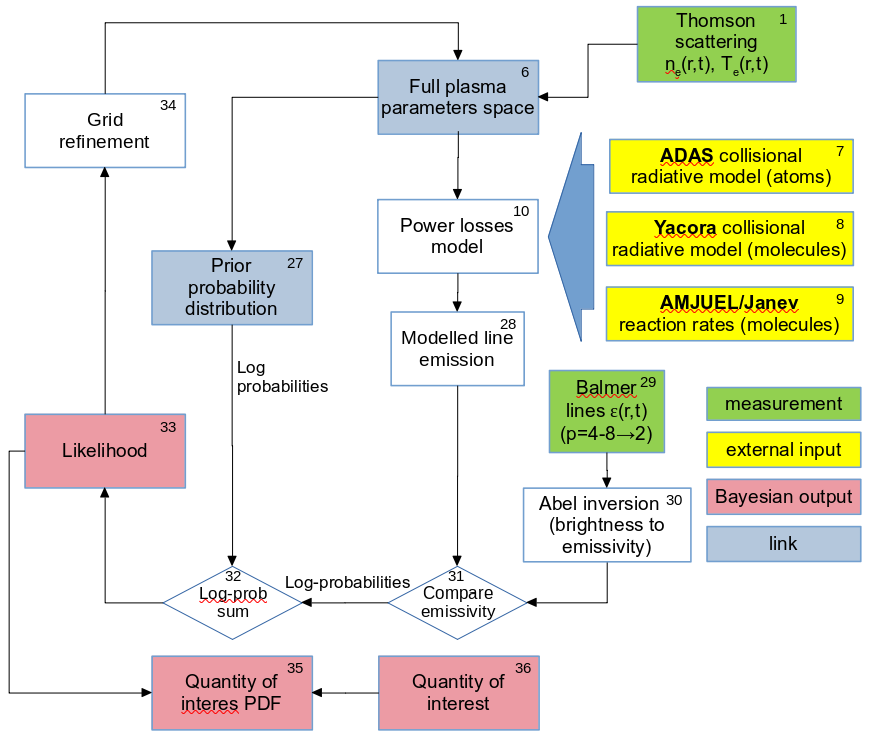
\includegraphics[scale=0.29,trim={0 0 0 0},clip]{Chapters/chapter3/figs/bayesian_steps13.png}
	\caption{Sketch illustrating how the likelihood distribution is determined comparing the line emission with the expected values and adding the prior log-probability, to refine the parameter grid and calculate the outputs PFD.}
	\label{fig:bayes1c}
\end{figure}


The expected value of the Hydrogen line emissivity is then compared with the measured one, and the resulting probability combined with the prior to return likelihood, also referred to as the sum of the Log-probabilities. The grid is refined twice around the regions of the grid with high likelihood to improve the resolution of the probability distribution. While keeping a grid structure requires a large amount of memory the numerical procedure is relatively simple.
This procedure is shown in \autoref{fig:bayes1c} and the meaning of the blocks here introduced is as follows:


\begin{enumerate}
    \item[29] \emph{Balmer lines $\epsilon(r,t)(p=4-8\rightarrow 2)$}: \\The Balmer line emission for transitions $(p=4-8\rightarrow 2)$ is measured with OES (see \autoref{Optical emission spectrometer}). The camera has a rolling shutter so it is necessary to decouple the line of sight from the time information, as detailed in \autoref{Sampling strategy} and \ref{OES data interpretation}.
    \item[30] \emph{Abel inversion (brightness to emissivity)}: \\Once the brightness per time step and line of sight is obtained an Abel inversion is operated (see \autoref{OES data interpretation}). The process converts the line integrated information to the local emissivity assuming poloidal symmetry and the plasma optically thin.
    \item[28] \emph{Modelled line emission}: \\As part of the power losses calculation the line emission from atomic and molecular processes the total line emission for the lines of interest ($p=4-8 \rightarrow 2$) is found (see \autoref{Emissivity}).
    \item[31] \emph{Compare emissivity}: \\The modelled line emissivity is compared to the measured one to return the probability that each combination of priors generated the measured emission (see \autoref{Emissivity}).
    \item[32,33] \emph{Likelihood}: \\The likelihood for every point of the parameter space is found adding the log probability from the prior and the comparison of the calculated emissivity with the measured one.
    \item[34] \emph{Grid refinement}: \\To increase the resolution in the region of the parameter space with high likelihood, the grid is refined by adding intermediate steps to the grid elements previously defined for every axis around the marginalised likelihood peak. The grid structure is maintained but it becomes non uniform. The prior probability distribution and comparison with measured emissivity is repeated to recalculate a new likelihood distribution. This loop is repeated twice to limit the computer memory requirements.
    \item[35,36] \emph{Quantity of interest PDF}: \\The quantity of interest for the plasma column power or particle balance have already been calculated for all the parameter space within \autoref{Prior probability distribution}. In order to reduce the size of the outputs the full range is reduced to a smaller number of intervals and the likelihood is summed within each interval.
\end{enumerate}


Once the PDFs for a quantity of interest in all radial and spatial locations are determined they are then convolved over radial steps, to obtain the total over the plasma column, and then in time over the ELM-like period to obtain the global quantities (see details in \autoref{Plasma column power balance}).

When a reaction occurs, energy is transferred between different species (e.g. plasma to molecules or atoms). If charged particles are created they are bound by the magnetic field and are confined to the same radial section of the plasma column. When neutral hydrogen atoms and molecules are generated they can escape the plasma column, carrying with them their kinetic energy. They can also interact with plasma at a different radii on the way out and  transfer the energy back in the plasma.

To model the transfer of energy to the neutrals and back to the plasma would require an effort beyond the scope of this work, so for now this component is not considered in the power and particle balance and only hyrdrogenic radiation is considered as net power leaving the plasma column. For more details see \autoref{Plasma column power balance}. 

It is important to address whether ignoring the power removed by the plasma column (and possibly transferred back) due to charge exchange (CX) and elastic collisions between $H_2$ and $H^+$ ($H_2$ elastic) is important and compatible with the Bayesian algorithm results. To estimate CX and $H_2$ elastic power losses we post-process our results as shown in \autoref{Power balance}. The same methodology was employed to reprocess B2.5-Eunomia results, and it returned a CX contribution between  a 1\% and 150\% and $H_2$ elastic within 18\% and 34\% of the correct (self consistent) values. In one instance, the simplified method produced a factor of 100 larger CX losses compared to B2.5-Eunomia result. It is observed that in this case, with both high temperature and density, a large fraction of the CX losses are recovered by fast neutrals exchanging back to the plasma their energy before escaping the plasma column. This behaviour can be captured by the Monte Carlo model but not by this simplified method. With these very large uncertainties it is possible to say that CX is likely more important than $H_2$ elastic for ELM-like pulses, contrary to what shown in \cite{Chandra2022}, but the relevance for the plasma column energy balance is uncertain and would require a more detailed analysis, out of the scope of this work.


\subsection{Analysis limitations due to restrictions on measured Balmer lines}\label{Limitations due to the measured lines}
While it is in general desirable to measure as many transition lines as possible, it became apparent during the setup of the experiment that the H$\alpha$ line ($p=3\rightarrow 2$) could not be measured simultaneously with lines $p\geq 4\rightarrow 2$ due to the grating used. We describe herein how the lack of the H$\alpha$ line prevents the separation of the line emission contribution from ${H_2}^+$ and ${H^-}$ precursors.

\begin{figure}[!ht]
	\centering
	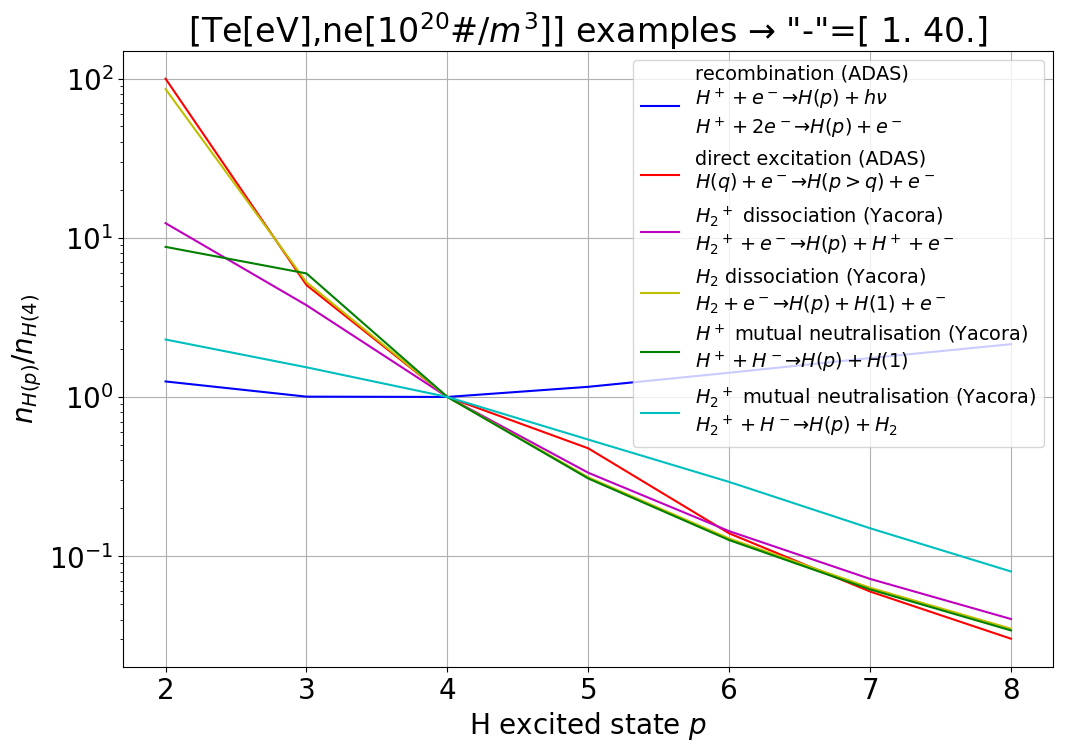
\includegraphics[width=0.7\linewidth,trim={0 0 0 36},clip]{Chapters/chapter3/figs/pure_rates_compare.png}
	\caption{Density ratio of hydrogen excited states to p=4 for different processes for typical $T_e=1eV,n_e=4 \cdot 10^{21}\#/m^2$ plasma. The similarity of the profile shape for ${H_2}^+$ dissociation and $H^+$ mutual neutralisation is maintained for all the $T_e,n_e$ range of interest.}
	\label{fig:lines1}
\end{figure}

As a reference, \autoref{fig:lines1} shows the density ratio of excited states produced by different processes with respect to p=4 for typical $T_e,n_e$ values. %The experimental setup unfortunately prevented the capability to measure $p=3\rightarrow 2$ line at the same time as the other Balmer lines due to the grating size. 
Restricting Balmer lines to $n \geq 4 \rightarrow 2$ recombination, ${H_2}^+$ mutual neutralisation and EIE have a distinctively different profile while ${H_2}^+$ dissociation, $H_2$ dissociation and $H^+$ mutual neutralisation are fairly similar. $H_2$ dissociation is usually not problematic because the $H_2$ density required to match the measured emissivity is excessively high. Conversely, ${H_2}^+$ dissociation and $H^+$ mutual neutralisation can be caused by relatively low molecular precursors densities, making it difficult to distinguish which caused the emission. This could have been alleviated by including $p=3 \rightarrow 2$ in the analysis\cite{Verhaegh2021a} but this was not possible with the available gratings. \autoref{fig:lines1} illustrates that with the present setup, using only the line ratios available is insufficient to distinguish which molecular precursor, ${H_2}^+$ or $H^-$, is dominant. This could be alleviated by combining matching line intensities with other conditions as described in \autoref{Analysis steps}, as it can help rule out regimes that can well match the emission profile but would be unphysical.

The results of this study and the relevance of molecular interactions during the ELM-like pulse will now be shown.

\subsection{Bayesian analysis results}\label{Bayesian analysis results}
In this section the results from the Bayesian analysis will be presented. The only show results regarding the strong pulse cases, since the temperature and density falls below the detection capabilities of the TS system for a significant fraction of the duration weak pulses.

\subsubsection{Power balance}\label{Power balance bayesian}
As explained in \autoref{Bayesian analysis} the results at each time and radial location are a collection of PDFs for the quantities of interest in the volume from target skimmer to target, like the power radiated via EIE. The temporal and spatial distribution of the most likely values can already be useful, as they can inform on the conditions in which some phenomena are important. Our inference show that ionisation and excitation tend to be more important close to the axis of the plasma column, where and when temperature is highest, but are not peaked on the axis as the atomic hydrogen density profile is hollow. Radiation from EIR is strong for high density and intermediate temperature. Radiation from excited H atoms ($H^*$) generated from plasma molecular reactions (PMR) is present at similar times and locations as EIR but is significant up to even larger radii (and lower temperatures) than EIR. This is shown for ID 10 in \autoref{tab:table1} in \autoref{fig:bayes_example_1}.

\begin{figure}[!ht]
	\centering
     \begin{subfigure}{0.48\linewidth}
    	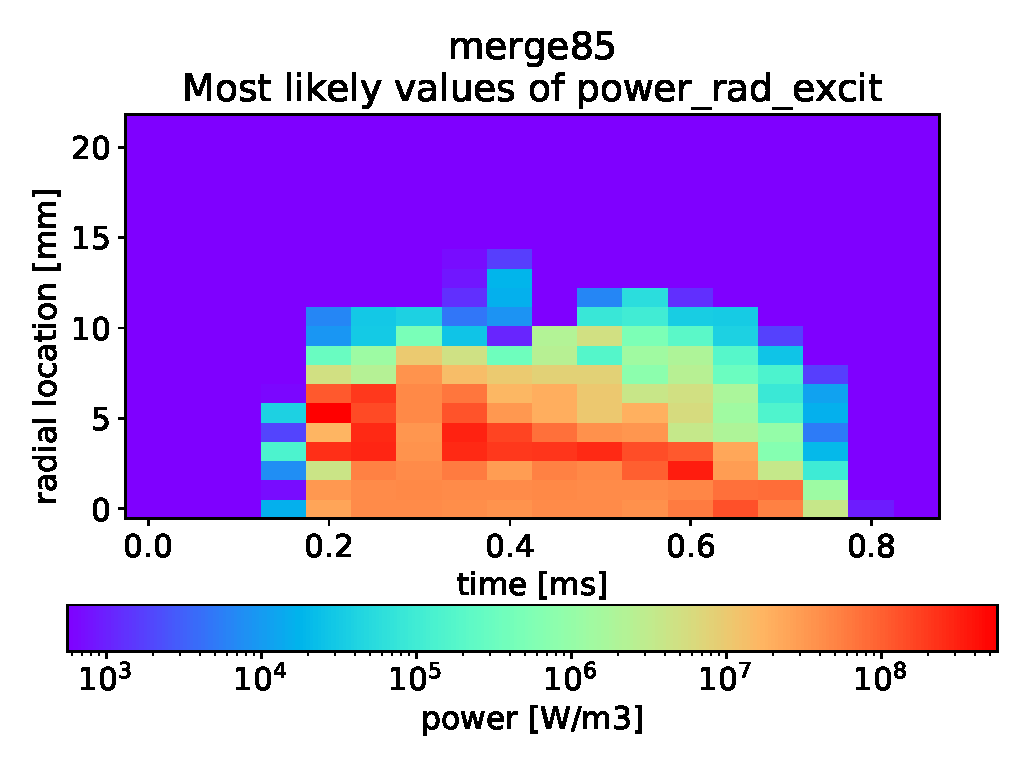
\includegraphics[width=\linewidth,trim={0 30 0 45},clip]{Chapters/chapter3/figs/_merge85_global_fit_example2.eps}
         % \vspace*{-5mm}
         \caption{radiated power EIE [$W/m^3$]}
        \label{fig:bayes_example_1a}
    \end{subfigure}
    \hfill
    \begin{subfigure}{0.48\linewidth}
    	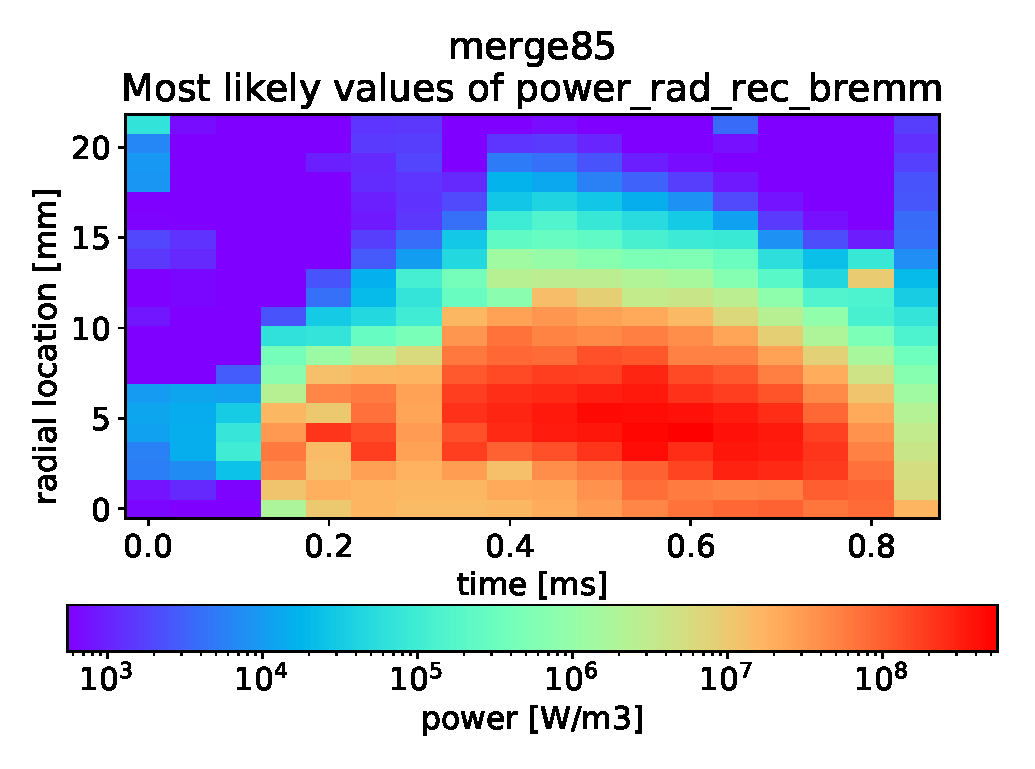
\includegraphics[width=\linewidth,trim={0 30 0 45},clip]{Chapters/chapter3/figs/_merge85_global_fit_example3.eps}
         % \vspace*{-5mm}
         \caption{radiated power recombination [$W/m^3$]}
        \label{fig:bayes_example_1b}
    \end{subfigure}
    \hfill
    \begin{subfigure}{0.48\linewidth}
    	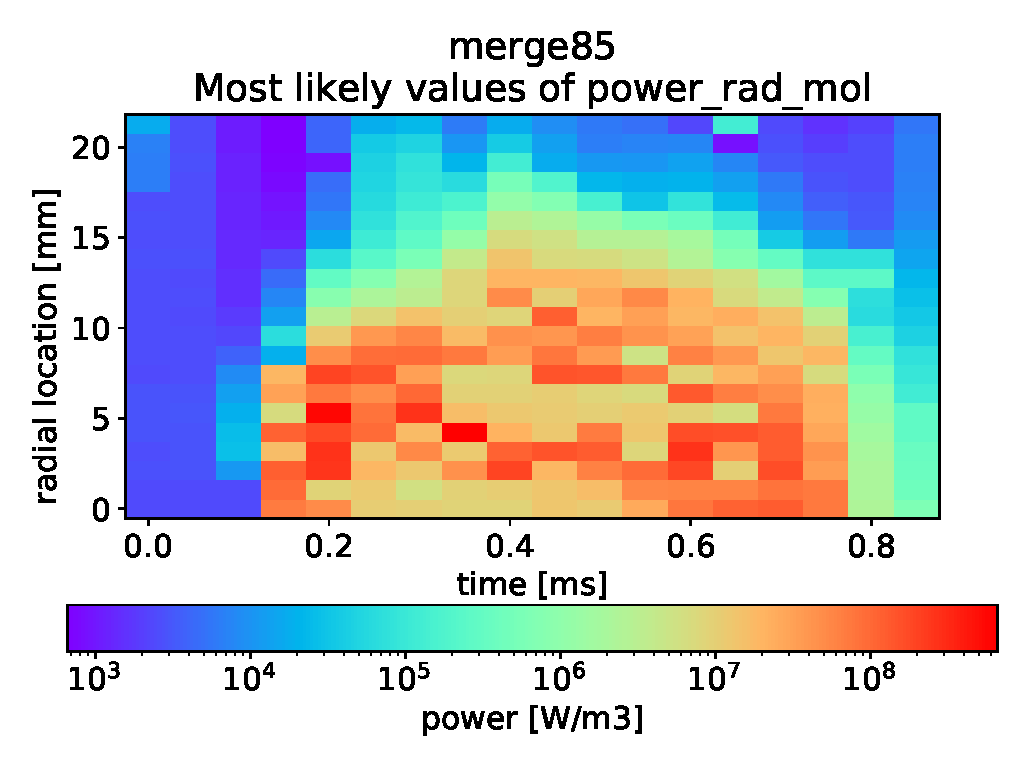
\includegraphics[width=\linewidth,trim={0 30 0 45},clip]{Chapters/chapter3/figs/_merge85_global_fit_example4.eps}
         % \vspace*{-5mm}
         \caption{radiated power MAR/MAI/MAD [$W/m^3$]}
        \label{fig:bayes_example_1c}
    \end{subfigure}
	\caption{Most likely values of the radiated power via EIE (\subref{fig:bayes_example_1a}), recombination (\subref{fig:bayes_example_1b}) and molecular processes (\subref{fig:bayes_example_1c}) for the same conditions of \autoref{fig:TSa}, ID 10 in \autoref{tab:table1}. The noise shown in these figures arise from the fact that the analysis is independent for   each radial and temporal location (no regularisation applied).}
    \label{fig:bayes_example_1}
\end{figure}

The PDFs are convoluved over the radial direction to integrate the parameter of interest on the radii. An example of the radial convolution of the power radiated from EIE at 0.4ms for ID 5 in \autoref{tab:table1} is shown in \autoref{fig:bayes_example_r_sum}. It can be noted that some PDFs, for example at $r=11mm$, show multiple peaks. This indicates that multiple possible combinations of the precursors densities with similar likelihood have been found.
\begin{figure}[!ht]
	\centering
	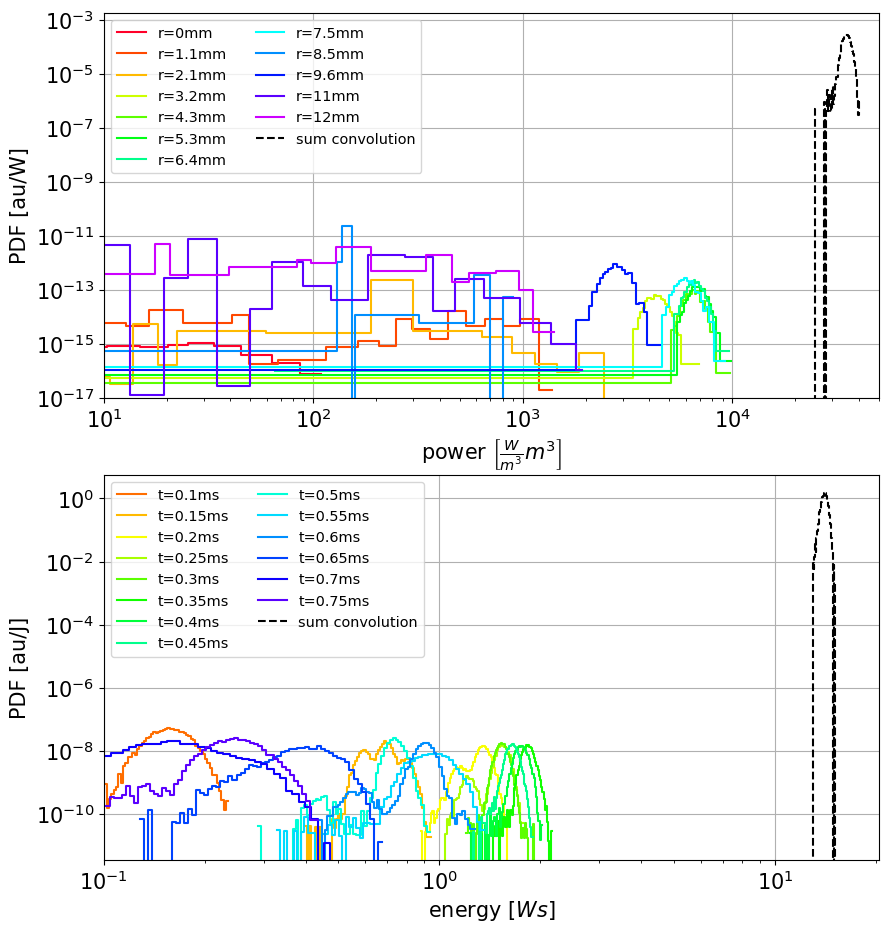
\includegraphics[width=0.9\linewidth,trim={0 332 0 0},clip]{Chapters/chapter3/figs/Bayesian_example_1.png}
	\caption{Example of the radial sum of the power radiated via excitation for ID 5 in \autoref{tab:table1} at 0.4ms. Only the radial locations that are more relevant are here shown. The power density ($W/m^3$) at each location is multiplied by the volume it pertains to determine the x coordinate.}
	\label{fig:bayes_example_r_sum}
\end{figure}

The evolution over time of the terms of the local the power balance, as per \autoref{Power balance}, are shown in \autoref{fig:bayes_example_2} for the lowest and highest pressure cases.
\begin{figure}[!ht]
	\centering
     \begin{subfigure}{1\linewidth}
        \centering
    	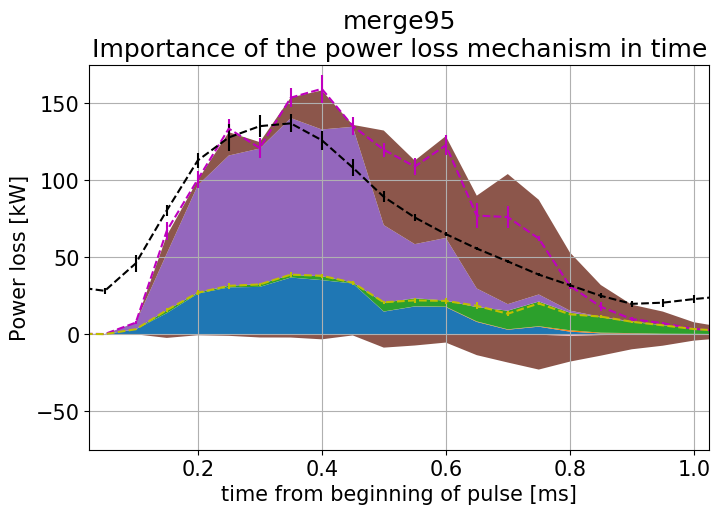
\includegraphics[width=0.7\linewidth,trim={5 0 5 45},clip]{Chapters/chapter3/figs/_merge95_global_fit_example44.png}
         % \vspace*{-5mm}
         \caption{neutral pressure = 0.3Pa}
        \label{fig:bayes_example_2a}
    \end{subfigure}
    \hfill
    \begin{subfigure}{1\linewidth}
        \centering
        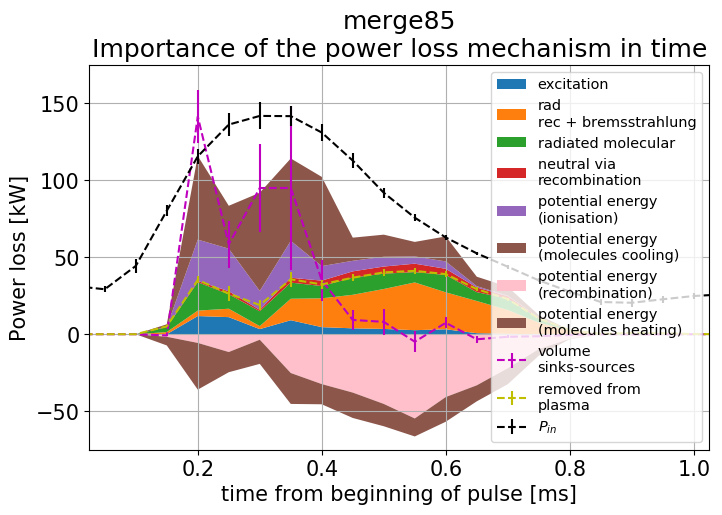
\includegraphics[width=0.7\linewidth,trim={5 0 5 45},clip]{Chapters/chapter3/figs/_merge85_global_fit_example7.png}
         % \vspace*{-5mm}
         \caption{neutral pressure = 15Pa}
        \label{fig:bayes_example_2b}
    \end{subfigure}
	\caption{Stacked area plot of the most likely values for the terms of the power balance as per \autoref{Power balance} for the lowest (\subref{fig:bayes_example_2a}) and highest (\subref{fig:bayes_example_2b}) pressure conditions for strong pulses. The data below zero corresponds to energy that released by recombination reactions heating the plasma. The potential energy from interactions with molecules is split in its positive and negative components. As \emph{molecules} is here intended any reaction different with exchange of potential energy different to EIR and ionisation. \emph{volume sinks-sources} corresponds to the the net local power balance while \emph{removed from plasma} indicates the contribution to the plasma column power balance as per \autoref{Plasma column power balance}. The colors in the legend of (\subref{fig:bayes_example_2b}) apply to both plots.}
    \label{fig:bayes_example_2}
\end{figure}
In \autoref{fig:bayes_example_2a} is shown that the energy of the ELM-like pulse is almost entirely used for ionisation, dissociation and molecular processes (MAD, MAI) increasing the plasma potential energy. However these ions recombine at the target, meaning that a larger fraction of the pulse energy will be able to reach the target, and in fact for this condition the target receives the most heat. The net power sink from the plasma is slightly larger than the input energy after its peak. This can be understood as there is no mechanism to enforce a global power balance since the analysis for every radial and temporal location is independent. The radiated energy is mostly due to EIE, that is to be expected due to the high temperature. After 0.6ms the temperature decreases below 4eV and the radiative and potential energy losses to the plasma from MAI/MAD and dissociation increases.
For higher neutral pressure (\autoref{fig:bayes_example_2b}) the peak in power input corresponds to the peak of power loss from molecular reactions rather than ionisation (due to the lower temperature) and most importantly, after the input power and temperature peak, there is a strong influence of EIR. Radiative losses and potential energy gains balance such that after 0.4ms the net power sink on the plasma is negligible.\cite{Verhaegh2019} The period of peak radiative losses now coincides with the peak in EIR. More energy is radiated then before and recombination in the volume means that the plasma is depleted before reaching the target. The radiative losses are on the expenses of the plasma potential rather than its thermal energy. This causes a reduction of the heat flux just like in deep detachment, matching with the results in \autoref{IR camera}. EIR dominates the path to radiative losses but the influence of molecular reactions increases.
These results are quite similar to recent studies of detachment in medium size tokamaks including molecular precursors.\cite{Verhaegh2022,Verhaegh2021}

The PDFs at each time are further convolved multiplying by the time interval they refer to, returning the total for the quantity of interest over the entire ELM-like pulse. In \autoref{fig:bayes_example_3} is shown how the total energy radiated by the plasma changes with target chamber pressure.
\begin{figure}[!ht]
	\centering
	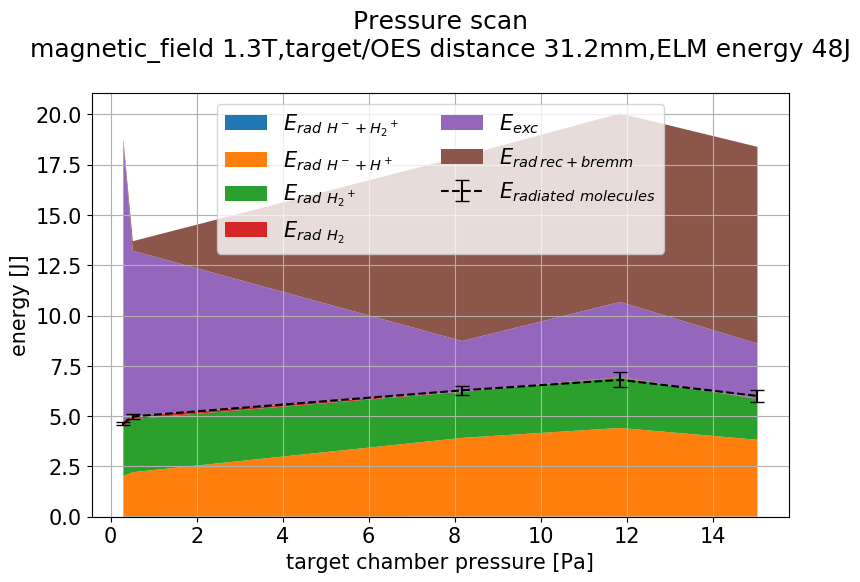
\includegraphics[width=0.7\linewidth,trim={0 0 30 60},clip]{Chapters/chapter3/figs/Bayesian_strong_4.png}
	\caption{Energy dissipated radiatively per mechanism for increasing neutral pressure (ID 5 to 10 in \autoref{tab:table1}) obtained with the Bayesian analysis.}
	\label{fig:bayes_example_3}
\end{figure}
As the target chamber pressure is increased (Stage 1 (P$<$2Pa) to 2 (P$>$2Pa)) the dominant process changes from EIE to EIR and the impact of molecules increases reaching up to $\sim$1/3 of the total radiated power. This is also reflected in the total radiated power in the visible wavelength range (not shown): in Stage 2 it is 3 times higher than in Stage 1, 0.3J and 0.1J respectively (the Lyman series is always responsible for most of the power radiated), largely due to the increase of EIR importance. This is not as a dramatic increase as observed in \autoref{fig:ELM2}, implying that the extrapolated $H\alpha$ emission, from our inferences, is overestimated. This could imply an overestimation of molecular assisted reactions could be in Stage 1 (visible radiated power losses due to EIE are 0.005-0.01J in for ID 5 and 6 in \autoref{tab:table1} respectively, with a better agreement with \autoref{fig:ELM2}). An overestimation of $H\alpha$ can also arise from an (over)underestimation of ($H^-$)$H_2^+$, changing the $H\beta/H\alpha$ ratio as shown in \cite{Verhaegh2020}. Among radiation due to molecules the precursor that is more important is $H^-$. This would be against results from previous analysis that show a dominance of the ${H_2}^+$ precursor\cite{Akkermans2020} but, as mentioned in \autoref{Limitations due to the measured lines}, the radiation from ${H_2}^+$ dissociation and $H^+$ mutual neutralisation has similar line ratios for the lines used in this study, so cannot be distinguished with certainty.

\begin{figure}[!ht]
    	% \includegraphics[width=\linewidth,trim={40 280 60 60},clip]{Chapters/chapter3/figs/bayesian_strong_3.png}
        \centering
    	\includegraphics[width=0.7\linewidth,trim={0 0 0 5},clip]{Chapters/chapter3/figs/bayesian_strong_3b.png}
	\caption{Results from the Bayesian analysis for strong ELM-like pulses with increasing neutral pressure (ID 5 to 10 in \autoref{tab:table1}). Total energy input (blue), energy removed from the plasma column (approximated with hydrogenic the radiative losses, red), energy absorbed by the target from IR camera analysis in \autoref{IR camera} (orange), estimated maximum energy removed from CX (gray) and $H_2$ elastic (black) collisions. CX and $H_2$ elastic have already been multiplied by the corrective factors found in \autoref{Bayesian analysis} by comparison with B2.5-Eunomia.}
	\label{fig:bayes2}
\end{figure}

In \autoref{fig:bayes2} are shown the variation of the terms in the global plasma column power balance with target chamber pressure. The energy absorbed by the target was determined in \autoref{IR camera}. The estimation of CX and $H_2$ elastic collisions is as per \autoref{Power balance}. The two terms are already multiplied by the corrective factors found by comparing their simplified model with B2.5-Eunomia, identified in \autoref{Bayesian analysis} (CX and $H_2$ elastic collision losses from B2.5-Eunomia being 1-150\% and 18-34\% respectively compared to the simplified estimate). The radiative energy losses increase with target chamber neutral pressure, up to $\sim$1/3 of the input energy, while the energy to the target decreases. This transition corresponds to the transition between Stage 1 and 2 introduced when analysing the visible fast camera brightness. $H_2$ elastic losses are of the same order of magnitude as radiative and target losses, while CX has a very large range from zero to one order of magnitude higher than $P_{in}$. These losses are here only estimated. Subtracting the radiative losses from the input energy returns much more than the measured target flux, allowing for other loss channels like CX, $H_2$ elastic collisions or the losses associated with plasma surface interactions, that are here not inferred.

From this very crude balance it seems that losses due to radiation and energy transfer to the target can account for about 1/3 of the input energy and $H_2$ elastic collisions for another 1/3. From fast camera observations, for high pressure conditions the energy dissipated at the target could be less relevant, leaving more room for CX losses, while the opposite for low pressure.

\subsubsection{Particle balance}\label{Particle balance bayesian}
During the experiment there was no direct measurement of any part of the particle balance, so it is not as well constrained as the power balance. Nevertheless thanks to the assumptions and approximations in \autoref{Balance over the plasma column} it is possible to perform a rough particle balance on the plasma column. Only the charged particles' particle balance is utilised, as only these are confined to a certain poloidal location by the magnetic field. Only $H^+, e^-$ are introduced by the plasma source, using the flow velocity estimated from the power input in \autoref{Balance over the plasma column}. The volumetric particle sources and sinks are calculated together with the power ones and the target particle losses are treated as an unknown in a similar way as in the power balance. To calculate the prior probability, the balance on $H^+$ and $e^-$ has a large uncertainty, as the plasma can potentially accumulate in the plasma column, while the balance on ${H_2}^+$ and $H^-$ has a smaller uncertainty due to their short lifetime. More detail on the particle balance is given in \ref{Particle balance}. 

The procedure to convolve the data from time and spatial dependent PDFs to a global one for the whole pulse is the same as previously mentioned for the power. In order to better understand the influence of molecular reactions on the plasma the individual reaction rates are divided in MAR, MAI and MAD. These are defined as the paths composed of a first reaction that converts a neutral specie ($H_2$, $H$) into a molecular precursor (${H_2}^+$, $H^-$) then a second one where the precursor is used. The final result of the two reactions combined can either be the recombination of the plasma that participated to the reactions (MAR) the ionisation of the original neutral (MAI) or the dissociation of $H_2$ (MAD). Here paths that cause ionisation or recombination and dissociation are not accounted in MAD to avoid double counting. All of the possible combinations of reactions that achieve the mentioned goals via a molecular precursor are added together to form the MAR, MAI and MAD rates.\cite{Verhaegh2020} 


\begin{figure}[!ht]
        \centering
    	\includegraphics[width=0.7\linewidth,trim={30 260 60 60},clip]{Chapters/chapter3/figs/bayesian_strong_6.png}
	\caption{Plasma particle balance on the plasma column from the Bayesian analysis for strong ELM-like pulses with increasing neutral pressure (ID 5 to 10 in \autoref{tab:table1}). Total particle input from the plasma source estimated from \autoref{Balance over the plasma column} and \ref{Particle balance} ($(nv)_{H^+,in}$). Number of plasma particles created during the duration of the ELM-like pulse by type of reaction. MAR and MAI are defined as ensemble of multiple reactions that, starting from neutrals, first create a molecular precursor (${H_2}^+$, $H^-$) then further react with the end result of the two consecutive reactions being plasma recombination or ionisation respectively.\cite{Verhaegh2020} We note that there can be a discrepancy between net$H^+$ and net$e^-$, wich appears to be an analysis artefact.}
	\label{fig:bayes3}
\end{figure}
The particle balance on the plasma is shown in \autoref{fig:bayes3}.
Here are shown the plasma particle input, constituted by the source, the ionisation source and the recombination sink. MAI increases at lower pressure but is not very important representing a small fraction of the total ionisation. With the considered reactions ${H_2}^+$ is the only precursor that can cause MAI. MAR increases with pressure, but it dominates at low pressure (high temperature), and amounts to $\sim$1/3 of the total plasma particle sink at high pressure (low temperature). It is mainly due to the $H^-$ precursor. 

An important observation is that for low pressure conditions the ionisation source is higher than the estimated particle input from the source. The main difference between linear machines and tokamak divertors is that in a divertor, especially in high recycling, most of the particle source for the plasma comes from the recycling neutrals while the upstream plasma acts as the energy source. Conversely in linear machines the external source usually dominates. For low pressure conditions this does not happen here. If the neutrals predominantly come from plasma recycling at the target surface, this might be evidence of recycling in a similar fashion as in a tokamak. %This could be supported by the observations with the fast camera in \autoref{Fast camera}.
\autoref{fig:bayes3} shows a decrease in net balance of protons and electrons in the plasma column (net$H^+$ and net$e^-$) for increasing neutral pressure due to a transition from an ionising to a recombining plasma. This is in agreement with both the analysis of power losses as per \autoref{Power balance bayesian} and the target heating analysis shown in \autoref{IR camera}. The potential energy exchanges in the plasma like ionisation, dissociation, MAI and MAD are important to lower the plasma temperature enough for MAR and EIR to become important and reduce the particle flux to the target. MAD is more efficient that electron impact dissociation (EID) in converting $H_2$ to $H$ and MAR can effect the plasma at higher temperature than EIR, therefore the inclusion of the chemistry from ${H_2}^+$ and $H^-$ is important in describing the ELM burn through processes.

\begin{figure}[!ht]
        \centering
    	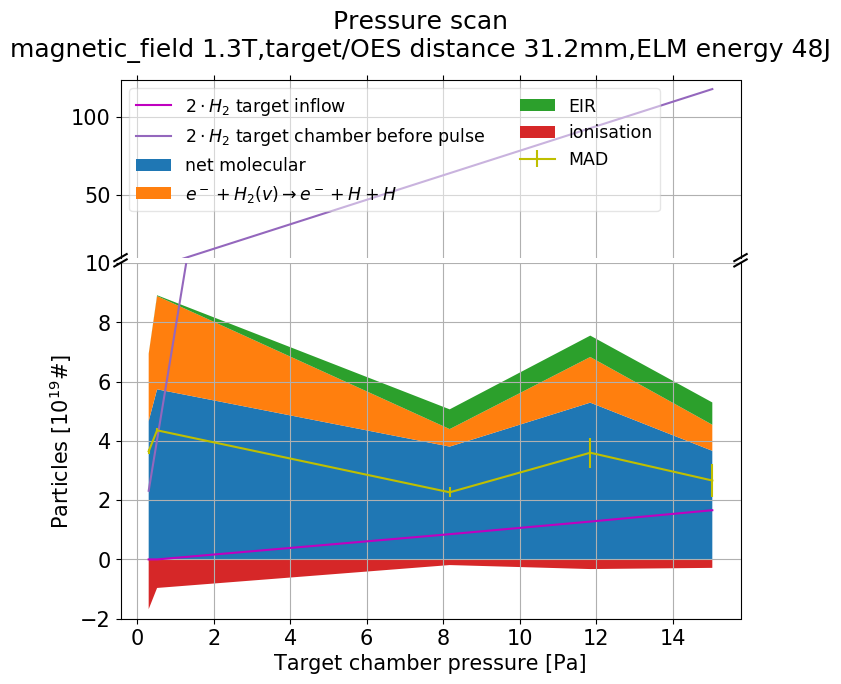
\includegraphics[width=0.7\linewidth,trim={35 5 60 50},clip]{Chapters/chapter3/figs/Bayesian_strong_7.png}
	\caption{Atomic hydrogen particle balance on the plasma column from the Bayesian analysis for strong ELM-like pulses with increasing neutral pressure (ID 5 to 10 in \autoref{tab:table1}). It is assumed no atomic hydrogen enters the plasma column from the source thanks to differential pumping so only volumetric sources/sinks and interactions with the surface (not inferred here) are possible. Number of particles created during the duration of the ELM-like pulse by type of reaction. MAD is defined as ensemble of multiple reactions that, starting from neutrals, first create a molecular precursor (${H_2}^+$, $H^-$) then further react with the end result of the two consecutive reactions being exclusively $H_2$ dissociation.\cite{Verhaegh2020}}
	\label{fig:bayes4}
\end{figure}

The particle balance for atomic hydrogen is shown in \autoref{fig:bayes4}. It must be kept into account that this balance is not directly constrained and that transport is not considered, so the balance is very tentative. Hydrogen from molecular reactions, and MAD within it, represent the largest contribution to the source. Considering also that MAI is less then 10\% of MAD reaction rate, this means that most of the power losses due to molecules in the local power balance (\autoref{fig:bayes_example_2}) are due to MAD. Molecular reactions are responsible (integrating the local power balance) for about half of the potential energy exchange while up to a third of the radiative power losses. Molecular reactions seem to not have a strong impact in the plasma particle balance while dominate the neutrals particle balance.

It must be noted that impact of molecular reactions on the particle balance, radiated power and potential energy is heavily dependent on the rates used. For this work the Yacora rates have been used to determine the radiative power losses due to molecular precursors. To determine the reaction rates and the potential energy losses other rates from AMJUEL and Janev have been used, with no guarantee of the consistency with Yacora (in terms of approximations used, consideration of different ro-vibrational states for $H_2$ and ${H_2}^+$ and other parameters used in the collisional radiative codes). For typical plasma conditions in this study ($T_e=2eV$, $n_e=10^{21}\#/m^3$), the average radiative power losses per molecular reaction are:
\begin{itemize}
    \item ${H_2}^+ + H^- \rightarrow H(p) + H_2$ : 0.17eV
    \item $H^+ + H^- \rightarrow H(p) + H$ : 8.2eV
    \item ${H_2}^+ + e^- \rightarrow H(p) + H(1)$ and \\ ${H_2}^+ + e^- \rightarrow H(p) + H^+ + e^-$ : 0.72eV
    \item $H_2 + e^- \rightarrow H(p) + H(1) + e$ : 0.026eV
\end{itemize}
The molecular rates are less established then atomic ones, so these numbers can change and significantly effect the power balance.


% \begin{itemize}
%     \item for ${H_2}^+ + H^- \rightarrow H(p) + H_2$ 0.17eV
%     \item $H^+ + H^- \rightarrow H(p) + H$ 8.2eV
%     \item ${H_2}^+ + e^- \rightarrow H(p) + H(1)$ \\ ${H_2}^+ + e^- \rightarrow H(p) + H^+ + e^-$ 0.72eV
%     \item for $H_2 + e^- \rightarrow H(p) + H(1) + e$ 0.026eV
% \end{itemize}

In low pressure conditions volume recombination is negligible and the vast majority of atomic hydrogen is produced by volumetric dissociation of $H_2$. Here the total volumetric source is higher then the total number of hydrogen atoms present in the target chamber before the ELM-like pulse and the neutrals that can be produced by surface recombination at the target (see \autoref{fig:bayes3}). This points to the source being over estimated, that can be expected being $H_2$ and $H$ particle balances not constrained. Both the hydrogen in the target chamber before the pulse and the possible neutrals generated at the target are larger then the volumetric ionisation sink. It is therefore unclear if what observed at low pressure is evidence of recycling or just dissociation and ionisation of a significant fraction of the gas in the target chamber.

The results from particle balances are here tentative and obtained with strong approximations, so further investigations will be necessary to better understand the respective roles of the various sources and sinks.


\section{Summary}\label{summary magnum-psi}

The effect of ELM-like pulses on a detached target in Magnum-PSI was studied with the help of various diagnostics. It was found that the ELM-like pulse energy can be effectively dissipated through high level of detachment before the ELM energy reaches the target. The decreasing power reaching the target is inferred to be due to higher volumetric power losses in the volume between target and source. The volumetric power losses, inferred from the visible light emission, for low neutral pressure are fairly constant along the magnetic field, presenting a strong peak close to the target due to plasma surface interactions indicating an attached plasma. The volumetric power losses become more uneven along field lines as neutral pressure is increased, with the region close to the target decreasing its brightness and expanding towards the plasma source. This change is correlated with increased loss of plasma before reaching the measuring location. This behaviour can be divided in stages. In Stage 1 the plasma is attached before and during the ELM-like pulse and the energy losses in the volume are at a minimum and predominantly not radiative. In Stage 2 the target chamber neutral pressure is such that the plasma is detached from the target in steady state but can reattach during the ELM-like pulse, and energy losses in the volume increase. Detachment during the steady state is correlated with a strong increase of the visible hydrogenic line emission, similar to what inferred from simulations.\cite{Zhou2022} In Stage 3 the plasma is detached before and during the pulse and the losses in the volume are such that the plasma cannot reach the target.

The power delivered to the target by the ELM-like pulse is independently calculated by measuring its temperature via an infrared camera. This dataset shows a reduction of the power to the target in agreement with the progress in stages. In the most extreme cases the power is not detectable, meaning the energy of the ELM-like pulse is completely dissipated in the volume. For the neutral pressure scan with strong pulses the heat flux factor, a metric often used to qualify the damage to the target given by ELMs pulses in tokamaks, is decreased by about half with increasing neutral pressure, becoming negligible at high pressure for weak pulses. This effect could be used in tokamaks, as they can have longer connection length between ionisation front and target and potentially similar neutral pressures, to reduce the risk of ELMs damaging the target.

The optical emission spectrometer was upgraded to acquire time and poloidally resolved brightness in the visible range. Dedicated routines were developed to separate the spatial and time dependence in the raw data given by the rolling shutter, and an Abel inversion was performed on the brightness to return the line emissivity. Hydrogen Balmer line emission from OES ($p=4-8 \rightarrow 2$) was used to develop a Bayesian routine that incorporates the results from multiple diagnostics to return the power balance in the plasma column in the target chamber. Various approximations to extrapolate the results from a single location in the target chamber to its entirety were adopted. The routine incorporates priors from numerical simulations (B2.5-Eunomia) and collisional radiative codes (Yacora, ADAS). The goal is to understand what drives the volumetric losses previously identified and what is the role of atomic and molecular assisted reactions.

It was found that radiation from the plasma due to molecular assisted reactions is an important but not dominant energy loss mechanism. Radiation from excited hydrogen atoms created from plasma molecular interactions is found to be the about the same for Stage 1 and 2, but this is likely due to overestimation in Stage 1. Mutual neutralisation of ${H}^-$ seems to dominate radiative losses, but it was established that this could not be determined from OES alone with the present setup. Molecular assisted reactions significantly effect the local plasma power balance exchanging kinetic to potential energy, limiting what is available for ionisation and recycling. This is somewhat analogous to tokamaks, where power limitation of the ionisation source can induce detachment\cite{Verhaegh2018}.



Molecular reactions predominantly lead to MAD, as it is a more efficient path to $H_2$ dissociation than EID. These losses could be here overestimated due to an unconstrained particle balance for $H_2$ and $H$. Molecular processes are mostly dominant in an intermediate temperature range around 3eV, between ionisation and EIR dominant regions. The radiated power losses can be responsible for significant plasma power losses, but exchanges of potential energy like ionisation, EID, MAI, MAD, and collisional processes like CX and $H_2$ $H^+$ elastic collisions are expected to dominate the plasma power balance. Ionisation is more important at high temperature, $>$5eV, while at lower temperatures MAD/MAR increases significantly. When these processes cause the the temperature of the plasma to go below $\sim$1.5eV EIR occurs, reducing significantly the plasma flow to the target and the relative heat flux. The importance of radiated power losses could be different if impurities like carbon or nitrogen are present. These results indicate that for highly detached regimes in linear machines molecular interactions are important and need to be accounted, something that is not yet fully done in many codes used for Tokamak edge plasma studies.
